% 编译：在 blueprint/notes 中运行
% latexmk -xelatex -outdir=../print/core-dag core-proof-dag-lean-roadmap.tex
\documentclass[UTF8,11pt,a4paper,fontset=none]{ctexart}
\usepackage[margin=25mm]{geometry}
\usepackage{fontspec}
\setmainfont{Latin Modern Roman}
\setmonofont{DejaVu Sans Mono}[Scale=MatchLowercase]
\setCJKmainfont{Noto Serif CJK SC}[AutoFakeSlant=.15]
\setCJKsansfont{Noto Sans CJK SC}
\setCJKmonofont{Noto Sans Mono CJK SC}
\usepackage{amsmath,amssymb,mathtools,amsthm}
\usepackage{array,booktabs,longtable,graphicx,tikz,xcolor}
\usetikzlibrary{arrows.meta}
\PassOptionsToPackage{obeyspaces}{url}
\usepackage[unicode,colorlinks=true,linkcolor=blue!50!black,urlcolor=blue!50!black]{hyperref}
\usepackage{xurl}
\usepackage{enumitem}
\setlist{itemsep=4pt,topsep=5pt}
\setlength{\parskip}{5pt}
\setlength{\parindent}{2em}
\emergencystretch=3em
\allowdisplaybreaks
\newcommand{\R}{\mathbb R}
\newcommand{\T}{\mathcal T}
\newcommand{\eps}{\varepsilon}
\newcommand{\mass}{\operatorname{mass}}
\newcommand{\vol}{\operatorname{vol}}
\newcommand{\N}{\mathcal N}
\DeclareRobustCommand{\id}[1]{\nolinkurl{#1}}
\newcommand{\lean}[1]{\par\noindent\textbf{Lean 声明：}\ {\small\path{#1}}\par}
\newcommand{\src}[2]{\par\noindent{\footnotesize 源文件：\path{#1}，第 #2 行起。}\par}
\newcommand{\node}[2]{\subsection{#2（\texorpdfstring{\id{#1}}{\detokenize{#1}}）}\label{node:#1}}
\newcommand{\arr}[2]{\id{#1}\,$\longrightarrow$\,\id{#2}}
\title{Blueprint 的 Core proof DAG：\\Roadmap、Lean 声明与实际依赖关系}
\author{}
\date{核对与定稿：2026 年 11 月 2 日至 3 日}
\begin{document}
\maketitle

这份说明讨论 blueprint 中名为 \emph{Core proof DAG} 的视图，即
\id{overview}。它有 18 个节点。比较的对象是这个视图的 Roadmap
连线、当前为各节点选定的 Lean 主声明，以及最终定理实际引用的声明。
这里的最终定理是 WZ2 Theorem 5.2 的离散体积估计；图本身不包括从它
推出 Hausdorff 维数或 Assouad 维数结论的后续论证。

先说明一个会影响全文的区别。图卡上写着论文定理的名字，不代表选中的
Lean 声明逐字实现了那个定理。选中的声明可能是定义，可能只是写出了一个
命题，也可能证明了带有额外条件的版本。另一方面，图卡之间少了一条线，
也不一定缺少一个数学步骤。一个引理可以接受已经给定的配置，而不调用
构造该配置的定理；这时构造定理和引理会一起被后面的定理使用。

当前最终证明在它明确写出的中间条件下成立。需要认真区别的地方包括：
Lemma 2.13 没有独立对应的 Lean 证明；WZ1 Theorem 5.2 的完整二择一
命题不是当前 C² 构造所调用的结果；Lemma 6.6 使用归一化的 slab 质量、
重数上界和相应准备；右边的投影下界使用归一化斜率以及长度 32 的粗管
测试。下面会把这些条件写出来，也会说明为什么它们没有变成最终
Theorem 5.2 的外加假设。

\tableofcontents

\section{怎样读这两个图}

\subsection{箭头方向、主声明和隐藏的步骤}

图中的 $A\to B$ 表示：$A$ 是 $B$ 的一个前提或组成部分。Lean 中保存的
引用方向相反：$B$ 的类型、证明或定义引用 $A$。例如图中 Proposition
6.5 指向 Lemma 6.7，而源码里是构造小投影的声明调用大斜率构造。

每张卡可以列出多个 Lean 版本，但画图使用一个选定的主声明
（\id{primary}）。判断箭头时比较的是两个主声明之间的路径，不能把
卡内另一个版本的证明移到主声明上。\id{W2L2_13} 的主声明为空；它的
数学卡片仍然保留在图上，但无法用它作为 Lean 路径的端点。

Lean 连线来自编译后保存的引用。提取器把没有单独显示的辅助声明折叠成
路径，又删去可以由其他可见路径表达的重复连线。因此一条线可能对应一次
直接调用，也可能对应七次引用。判断一条 Roadmap 线有无对应关系时，要
检查完整路径，不能只找一次直接调用。

还有两类引用需要区别。一个定理的证明使用另一个定理，这是证明依赖。
一个配置的类型包含 CWA 条件，或者定理的类型提到了极端配置，这首先是
定义或数据的依赖。Lean 图会把后一类画成 API 线。它说明陈述需要该定义，
不能被解读成“这里又证明了一次定义所描述的结论”。

\subsection{线型和比较结果是两件事}

两层图沿用同一套线型：实线表示证明依赖，灰色虚线表示定义、API 或通常
的操作，紫色点划线表示把一个输出组装成下一个输入，紫色长虚线表示隐藏了
中间步骤。线型描述用途，不直接表示两张图是否一致。

比较器另有 \emph{agree}、\emph{Lean only}、\emph{Lean detail} 和两类
\emph{roadmap only} 结果。这里的 \emph{agree} 只要求 Roadmap 也有从
前提到结论的路径，不要求它画出同一条直接连线。用来比较的是包括详细视图
在内的完整 Roadmap。因此，一条在 Core 图里新出现的 Lean 线仍然可能
被标为 \emph{agree}。

本次核对的数字很具体：Roadmap 有 17 条线，Lean 层也有 17 条线，两层
共有 12 对端点。Roadmap 中其余 5 条线的情况是：2 条涉及没有主声明的
Lemma 2.13，2 条在两个已使用的主声明之间没有依赖路径，1 条涉及未进入
最终证明的 WZ1 命题接口。Lean 新画出另外 5 对端点。当前 Core 视图没有
被比较器标为 \emph{Lean only} 的连线；这并不意味着两层画法完全相同。

\subsection{本文怎样使用 literal 这个词}

本文所说的“不是 literal”，是指不能把图卡的自然语言当作选中 Lean
声明的逐字数学陈述。这个问题至少有四种不同情形：没有独立对应声明；
只有命题定义而没有该命题的证明；证明的适用范围与图卡不同；同一数学
操作在 Lean 中保存了更多构造数据。它们不能合并成一个“未完成”标签。

定义本来就应该由定义声明对应。例如 CWA 和极端配置的节点是定义节点，
不需要被误判为缺少存在性证明。对这些节点需要检查的是定义内容是否对应，
以及参数和量词是否相同。后面的逐节点说明分别处理这些问题。

\section{把 Lean 中的对象写成论文常用的记号}

\subsection{管族、shading、质量和体积}

把 \id{TubeFamily delta} 写成有限的、带指标的 $\delta$-管族
$\T=(T_i)_{i\in I}$。指标在这里有作用：不同单位线段可以有相同的
支撑直线参数。计数时必须数指标，不能先把相同参数合并。把
\id{TubeShading family} 写成 $Y=(Y_i)_{i\in I}$，其中 $Y_i\subset T_i$。
普通分析模型中的 $T_i$ 是单位线段的闭 $\delta$ 邻域；第 6 节构造还用到
论文管体及其 cubical shading，转换时会保留包含关系和质量估计。

记
\[
 E_Y=\bigcup_{i\in I}Y_i,\qquad
 \mass(Y)=\sum_{i\in I}|Y_i|,\qquad
 \mu_Y(p)=\#\{i:p\in Y_i\}.
\]
质量会重复计算同一点上的多个指标，$|E_Y|$ 则只计算并集体积。
\id{IsLambdaDense Y lambda} 的意思是
\[
 \mass(Y)\geq\lambda\sum_{i\in I}|T_i|.
\]
这是总体密度条件，不要求每个 $Y_i$ 都达到密度 $\lambda$。源码用
\id{ENNReal} 容纳非负数和无穷值，\id{realRpowENN delta a} 就是把
$\delta^a$ 放进这个类型。翻译成数学语言时保留 $\delta>0$，然后直接写
$\delta^a$；不用把类型转换也搬进论文。

\subsection{几种不集中条件}

论文形式的 CWA 要求，对每个凸集 $K$，
\begin{equation}\label{eq:body-cwa}
 \#\{i:T_i\subset K\}\leq C|K|\#\T.
\end{equation}
普通分析版本 \id{ConvexWolffBound} 保留了固定单位管体积的归一化：右边为
$C(|K|/v_1)\#\T$，其中 $v_1$ 是 \id{deltaTubeVolume 1}。源码证明
$v_1\geq1$，因而这个分析版本直接给出式~\eqref{eq:body-cwa} 的较弱形式。
在固定模型之间比较时，这个差异是固定常数；在逐字陈述时则应保留它。

普通 Tube Wolff 只用普通单位线段粗管 $U_r$ 作测试，把
式~\eqref{eq:body-cwa} 中的 $K$ 换成 $U_r$。长度 32 的版本则用粗管的
中心 32 倍放大作测试。细管仍是原来的单位线段管；改变的是测试集合。
若原粗管半径为 $s$，放大后的轴长为 32、物理半径为 $32s$。
这不是只把轴长改成 32 而保留 $s$ 不变的定义。

“本质不同”也有两种具体定义。公共附近尺度条件使用普通论文定义：
对不同指标 $i,j$，$T_i$ 不包含在 $T_j$ 的中心 2 倍放大中，反向
包含也不成立。分析最终配置的 \id{IsEssentiallyDistinct} 则要求
\[
 |T_i\cap T_j|\leq\tfrac12\max(|T_i|,|T_j|)\quad(i\ne j).
\]
在 $0<\delta\leq1/100000$ 时，已证明的
\id{WZ2PaperOrdinaryIsEssentiallyDistinct.overlapDistinct} 从普通
论文定义推出分析的交集体积条件。另一些去近管选择则直接保证所选子族
具有所需分析证书。这里没有一个不带尺度条件的双向等价声明。
后面的 packing 和普通单位球版本应使用各自声明实际要求的证书。
\src{MyLeanRepo/Kakeya/Assouad/PureWZ2/OrdinaryDistinctToOverlapDistinct.lean}{618}

在竖直坐标图中，支撑直线写成
\[
 (x,y,z)=(a_i+c_i z,\ b_i+d_i z,\ z),\qquad
 p_i=(a_i,b_i,c_i,d_i).
\]
\id{TubeParameterFrostmanBound F C} 的逐字意思是：对每个
$\delta\leq r\leq1$ 和每个参考指标 $j$，
\begin{equation}\label{eq:parameter-frostman}
 \#\{i:\|p_i-p_j\|_\infty\leq r\}
       \leq Cr^2\#\T.
\end{equation}
它数的是参数附近的所有指标。一个细管的支撑直线参数靠近参考管，并不
意味着它的整个单位线段被参考管的一段单位粗管包含；线段可以沿支撑直线
移动。这正是后面 Proposition 7.1 的区别所在。

一维 AD 条件在这里也是上界。集合 $A\subset\R$ 为
$(\delta,\alpha,C)_1$-ADset 的含义是，对所有
$\rho\geq\delta$ 及所有长度 $L\geq\rho$ 的区间 $J$，
\[
 \N_\rho(A\cap J)\leq C(L/\rho)^\alpha.
\]
$\N_\rho$ 是用半径 $\rho$ 的球覆盖所需的数量。这个条件没有一条对应的
下界，不能翻译为双侧 Ahlfors--David 正则性。

\subsection{斜率、坐标图和扭曲投影}

\id{SlopeFunction} 是一个定义在整条实轴上的 $C^2$ 代表。
\id{IsNormalized} 要求在 $[-1,1]$ 上
$|f|,|f'|,|f''|\leq1$；\id{IsNonsingular} 则要求
\begin{equation}\label{eq:nonsingular}
 1\leq|f'(z)|\leq2,\qquad |f''(z)|\leq1/100.
\end{equation}
后一个条件没有规定 $f(0)$，也没有规定 $|f|\leq1$。
源码中额外的 \id{f 0 = 0} 应译成 $f(0)=0$，不能藏进“非退化斜率”这个
称呼。由它和式~\eqref{eq:nonsingular} 才能得到 $|f(z)|\leq2$。

\id{HasBoundedBase F 4} 是每根管的起点范数不超过 4。
\id{IsInVerticalChart F} 是每个单位方向向量 $v_i$ 的竖直分量满足
$|(v_i)_z|\geq1/2$。它不要求不同方向彼此分离。
\id{IsInSlopeWindow Y} 是 $E_Y\subset\R^2\times[-1,1]$。

扭曲投影及其并集写成
\[
 \pi_f(x,y,z)=(x+f(z)y,z),\qquad X_f(Y)=\bigcup_i\pi_f(Y_i).
\]
这里 $|X_f(Y)|$ 是平面面积。Lean 中的 \id{twistedUnion Y f} 就是这个
集合。投影前后的体积处于不同维数，阅读后面的 Jacobian 时要分别处理。

\section{设置和极端配置：前五个节点}

\node{W2MW}{WZ2 Definition 2.12：每个尺度的 CWA}
\lean{Kakeya.Assouad.WZ2PaperPureCWAAtNearbyScales}
\src{MyLeanRepo/Kakeya/Assouad/PropStickyDefinition2_12.lean}{703}

这个声明定义一个命题。翻译后是：$\delta>0$，误差常数 $A$ 是有限的
允许常数，普通管族本质不同。对每个请求尺度
$\rho_0\in[\delta,1]$，存在实际尺度 $\rho$，使
\[
 \rho_0\leq\rho<A\rho_0,
\]
并有相应的 $\rho$-管覆盖、完整包含纤维的一致性以及每个纤维的单位
重缩放 CWA 证书。完整纤维是包含在该父管内的全部细管，不是调用者可以
另外挑选的某一部分。覆盖的 partitioning 条件和 full-fiber 条件一起保存
了第 2.12 定义要求的父子关系。

更具体地，若 $I_U=\{i:T_i\subset U\}$，完整纤维的一致性要求任意
两个父管满足 $\#I_U\leq A\#I_{U'}$。误差常数满足 $1\leq A<\infty$。
每个纤维的重缩放通过父凸体的单位归一化给出，重缩放后的子体仍有
误差 $A$ 的 CWA。声明保留这些实际几何数据，而不只是一个指派的
父指标函数。

这基本对应 Roadmap 的根假设，但两点值得逐字核对：上界是严格的
$\rho<A\rho_0$；只有请求尺度 $\rho_0$ 被限制在 1 以内，实际尺度
$\rho$ 可以超过 1。不能在翻译时默默加上 $\rho\leq1$。这个节点不提供
方向分离条件，也不预先提供每个尺度精确相同的子管数。

\node{W2L2_13}{WZ2 Lemma 2.13：粗细尺度的继承}

Roadmap 在这里写的是一个一般继承引理：给定每尺度 CWA，可以在所需的
附近尺度选覆盖，使粗族和单位重缩放后的每个细纤维仍满足多尺度条件，误差
为 $O(A)$。图还用 partitioning 解释连续尺度上的纤维如何形成嵌套树。

当前映射中 \id{primary} 为空，\id{lean} 列表也为空。因此这里没有可以
翻译成论文语言的独立 Lean 定理。正文不能写成“Lean 已证明 Lemma
2.13”，更不能从这张卡推断任意精化都保留所有尺度的 CWA。

实际结构构造会为它使用的覆盖和纤维重新建立所需证书。这个做法足以支持
当前构造，但不能被替换成上面那个一般继承陈述。这也解释了为什么
\arr{W2MW}{W2L2_13} 和 \arr{W2L2_13}{W2P6_2} 在 Lean 层没有
对应线：中间节点没有独立声明，不是提取器漏掉了一个同名调用。

\node{W2Sigma}{WZ2 Section 6.2：临界指数}
\lean{Kakeya.Assouad.PureWZ2Admissible}
\lean{Kakeya.Assouad.pure_wz2_node02_critical_extraction}
\src{MyLeanRepo/Kakeya/Assouad/PureWZ2/Core.lean}{45}
\src{MyLeanRepo/Kakeya/Assouad/PureWZ2/Critical.lean}{262}

图卡用 $\sigma_{\rm CW}$ 表示一个上确界。主声明却是一个接受实数
$s$ 的谓词：对任意 $\eta>0$ 和 $\delta_0>0$，都存在
$0<\delta\leq\min(\delta_0,1)$、非空管族和 shading，满足每尺度 CWA
误差 $\delta^{-\eta}$、总体密度 $\delta^\eta$，并且
\[
 |E_Y|\leq\delta^s.
\]
也就是 Roadmap 所说的 $\mathsf{Bad}(s)$。这个定义本身既不是一个数，
也不是 $\sigma>0$ 的证明。

真正的临界提取结果接受已证明的 subunit 体积下界和最终定理失败的假设，
返回某个 $0<\sigma<1$。连同它返回的 \id{PureWZ2CriticalPackage}
有两项主要性质。第一，对任何正损失和任何正尺度上限，都有更小尺度的
极端配置。第二，对任何 $a>0$ 和允许的结构损失上限，先能选
$\eta>0$ 及 $\delta_0>0$，使相应的非空 CWA 配置统一满足
\[
 |E_Y|\geq\delta^{\sigma+a}.
\]
提取证明内部取上确界；仓库没有另行导出一个全局常数
$\sigma_{\rm CW}$，也没有把它与 WZ1 方向模型的 $\sigma_3$ 识别。

因此这张卡不是 literal 的地方是“一个全局临界常数”与“一个可接受指数
谓词加局部提取过程”的对应。数学目的相同，但声明不同。图中的
\arr{W2Sigma}{W2D6_1} 也不会自动出现：下一张卡的定义接受任意显式
参数 $\sigma$，不需要引用这个可接受指数谓词。

\node{W2D6_1}{WZ2 Definition 6.1：极端配置}
\lean{Kakeya.Assouad.WZ2PaperPureIsExtremal}
\src{MyLeanRepo/Kakeya/Assouad/PropStickyDefinition2_12Extremal.lean}{41}

给定实数 $\sigma,\eta$、尺度 $\delta$、管族 $\T$ 和 shading $Y$，
这个结构命题表示
\[
 \begin{gathered}
 0<\delta\leq1,\qquad\T\ne\varnothing,\qquad
 \T\text{ 有每尺度 CWA，误差 }\delta^{-\eta},\\
 \mass(Y)\geq\delta^\eta\sum_i|T_i|,\qquad
 |E_Y|\leq\delta^{\sigma-\eta}.
 \end{gathered}
\]
它是这些条件的集合，不是极端配置存在性定理。存在性放在上一节的临界
package 中。图卡把 $\sigma$ 约定为临界指数，Lean 定义则允许显式输入
任意 $\sigma$；在实际调用中才传入临界 package 的指数。

这里的 shading 密度与 Roadmap 一样是平均条件。非空性和
$0<\delta\leq1$ 写得更明确。不要把它翻译成每根管的逐管密度，也不要
在定义中增加 WZ1 的方向覆盖假设。Lean 从本节点到 Proposition 6.2
的那条线首先是输入类型中使用极端配置定义的 API 关系。

\node{W2P6_2}{WZ2 Proposition 6.2：平衡的粗细极端结构}
\lean{Kakeya.Assouad.pure_wz2_node03_rich_prop62_kernel}
\src{MyLeanRepo/Kakeya/Assouad/PureWZ2/Prop62RetainedKernel.lean}{16}

Roadmap 把它写成一个运行时陈述：给定足够极端的细配置和
$\delta^{1-\eps}\leq\rho\leq\delta^\eps$，得到精化、平衡的粗覆盖以及
重缩放后的极端纤维。它保留的典型上界为
\[
 \#\T_\rho(p)\leq\rho^{2-\sigma-\eps}\#\T_\rho,
 \qquad
 \#\T'[U](p)\leq(\delta/\rho)^{2-\sigma-\eps}\#\T'[U].
\]
这里的族基数因子是 WZ2 陈述的一部分，不能用方向分离的直觉删掉。

当前主声明证明的形式是：给定正临界 package 和任意
$0<\alpha\leq1$，存在一套在运行时数据之前选定的损失和尺度界。这套
数据选定源损失 $\eta_{\rm src}$、归一化损失 $\eta_{\rm norm}$ 和
$\delta_0>0$，其中
\[
 0<\eta_{\rm src}\leq\eta_{\rm norm}/2,
 \qquad 0<\eta_{\rm norm}<\alpha.
\]
源损失还满足源码给出的归一化损失关系。随后，给定
$0<\delta\leq\delta_0$、裁剪的论文模型 shading、它的
\id{PureWZ2PropStickyReentryData}，以及
$\delta^{1-\alpha}\leq\rho\leq\delta^\alpha$，这套数据的运行函数返回
相应的粗细结构。

这里的 re-entry 数据不是一个任意名字。它保存裁剪后的配置和普通配置
之间的几何转换及极端性、CWA、密度等条件，使粗配置可以再被下一次结构
构造使用。主声明所返回的较强版本还保存最终配置的实际粗细对象、重数证书、
普通归一化和再次使用的条件。Proposition 6.3 的两次结构调用正需要这些
数据。若忘掉它们，只留下老的公开输出，就不能从该输出反向恢复原来的
构造过程。

因此这张卡的数学内容不是“有一个名字与 Proposition 6.2 相同的定理”
这么简单。它选中的是带有运行函数的较强构造，输入也明确保留模型准备。
老的 \id{pure_wz2_node03_prop_sticky} 接受 subunit 和 critical-extraction
两个前提，返回后续可调用的数据；它不是一个无参数的独立存在性结果。
当前入口把这些前提的已证明版本传进去。这与最终定理不接收外部
证明参数是相容的。

\section{从 grains 到 C²：三个节点及 WZ1 的外部输入}

\node{W2P6_3}{WZ2 Proposition 6.3：全局和局部 grains}
\lean{Kakeya.Assouad.pure_wz2_node04_reentrant_grains}
\src{MyLeanRepo/Kakeya/Assouad/PureWZ2/Grains/ReentrantEntry.lean}{18}

论文语言的输出是：任意给定正损失和尺度上限，都可得到一个更小尺度的
极端配置、一个 $1$-Lipschitz 的全局斜率 $f:[-1,1]\to\R$，以及一个
$1$-Lipschitz 的局部单位法向场 $V$。对每个固定高度 $z$，
\[
 \{x+f(z)y:(x,y,z)\in E_Y\}
\]
满足一维 $(\delta,1-\sigma,\delta^{-\eps})_1$-AD 上界。对每个
有效局部中心 $p$ 和每个 $\delta\leq\rho\leq1$，
\[
 \{V(p)\cdot q:q\in E_Y\cap B(p,\sqrt\rho)\}
\]
满足 $(\rho,1-\sigma,\delta^{-\eps})_1$-AD 上界。

有一个量词区别必须讲清楚。Roadmap 简写了“所有 $p$”，Lean 中
\id{planeMap} 的定义域是 $E_Y$ 上的点，即 $p\in E_Y$。它还保留
$\|V(p)\|=1$ 和管方向的入射关系。调用者若想在一个网格方块中心评价
$V$，先要证明中心属于定义域，或者选一个实际被占据的锚点；不能直接
把它当成整个 $\R^3$ 上已经给定的函数。

主声明另接受 Proposition 6.2 所构造的调用数据
\id{capability}。给定临界 package、输出损失 $\alpha>0$ 和源尺度上限，
它返回 $0<\eta<\alpha$ 和更小的源尺度，连同一份依赖于同一族和
shading 的 grains 与普通／裁剪 re-entry 数据。这份较强数据进入 C²
层次构造。忘掉 re-entry，并放宽损失，即得到老的论文输出；管族、
shading、全局斜率和局部法向场在这个投影中没有重新选择。

\arr{W2P6_2}{W2P6_3} 是一次实际证明调用：grains 入口把
\id{pure_wz2_node03_rich_prop62_kernel} 传入它的构造函数。不是只借用
一个损失数字，也不是给结构体加一个“来自 Proposition 6.2”的标记。

\node{W2P6_4}{WZ2 Proposition 6.4：C² 全局斜率}
\lean{Kakeya.Assouad.pure_wz2_left_line_c2_grains}
\src{MyLeanRepo/Kakeya/Assouad/PureWZ2/LeftLine.lean}{35}

这个入口的陈述可写成：给定正临界 package，对任意
$\alpha>0$ 和 $\delta_0>0$，存在 $0<\delta\leq\delta_0$ 以及同一个
配置上的全局和局部 grains。全局斜率有 $C^2$ 代表，满足
\[
 |f(z)|,\ |f'(z)|,\ |f''(z)|\leq1\quad(z\in[-1,1]),
\]
全局和局部 AD 上界的误差为 $\delta^{-\alpha}$。

Lean 的输出比图卡多保存了第 6 节使用的模型条件：有界起点、论文的直线
坐标类、cubical shading、裁剪模型极端性，以及顶层 CWA。全局 grains
和局部 grains 均以同一份 shading 为参数。源码里的组合选择不会分别给
两种 grains 选出两份无法比较的配置。

入口先从已证明的 Proposition 6.2 调用数据出发，再把实际的
\id{pure_wz2_node04_reentrant_grains} 输出传给
\id{pureWZ2_c2_grains_from_reentrant}。所以
\arr{W2P6_3}{W2P6_4} 有直接引用。图卡里的 WZ1 Section 5 路线仍然
有数学作用，但其完整二择一定理不是这个入口调用的声明，下一小节展开
这个区别。

仓库还构造了一份带全局细管重数上界的 C² 来源；这份重数来源被实际
Proposition 6.5 构造使用。另外有一个独立的 prescribed-intervals
入口：先固定这份配置，再对后来给定、满足归一化质量和覆盖条件的每个
$J$ 调用归一化 Lemma 6.6。它不重新选择 C² 配置，并在每个 slab
内部证明框架相容性。

当前根证明没有调用这个 prescribed-intervals 入口和任意配置的
normalized interval 定理；它仍通过准备版 Lemma 6.6 构造
Proposition 6.5。应分别看待“全局细管重数来源被使用”和“任意区间
兼容入口已证明但未被该根调用”。这里先固定配置、再处理所有后来的
$J$，也与每给一个 $J$ 都重新选择配置不同。

\node{T5_2}{WZ1 Theorem 5.2：点积展开或直线集中}
\lean{Kakeya.Assouad.WZ1ProjectionDichotomyConclusion}
\src{MyLeanRepo/Kakeya/Assouad/WZ1/Statements.lean}{1105}

图卡在这里是一个外部数学定理。它的 Lean 主声明只定义了一个命题，
并没有证明这个完整命题。这个声明不在最终根定理的依赖闭包中。

把命题本身翻译出来，Lean 使用三个非空、$\delta$-分离的有限点集
$F,G_1,G_2\subset B(0,1)\subset\R^2$，每个都满足维数 1 的绝对
Katz--Tao 计数上界，误差 $\delta^{-\eta}$。它要求以下二择一。

第一种情形：存在单位方向 $v$ 和点 $b$，使 $F$ 在过原点的方向
$v^\perp$ 直线附近有至少 $\delta^{\eps-1}$ 个点，而 $G_1$ 和 $G_2$
\emph{各自}在同一条仿射直线 $b+\R v$ 附近有至少这么多点。

第二种情形：对\emph{每一个} $H\subset F\times G_1\times G_2$，
只要 $\#H\geq\delta^{\eta-3}$，就存在 $\delta\leq\rho\leq1$ 和
正长度区间 $J$，使 $|J|\geq\delta^{-\eta}\rho$，且
\[
 \N_\rho\bigl(J\cap\{a\cdot(b_1-b_2):(a,b_1,b_2)\in H\}\bigr)
       \geq(|J|/\rho)^{1-\eps}.
\]
Lean 用球心 \id{center} 和半径 \id{radius} 表示这段闭区间，所以
长度 $|J|$ 是半径的两倍；长度条件在源码中写成
$\delta^{-\eta}\rho\leq2R$，其中 $R$ 是 \id{radius}。
Roadmap 使用一个端点集 $G$，Lean 区分 $G_1,G_2$。此外，卡片原
集中式把 $F$ 放在仿射线 $\ell$ 附近，把 $G$ 放在过原点的
$\ell^\perp$ 附近；Lean 对 $a\cdot(b_1-b_2)$ 所用的方向恰好相反：
系数集 $F$ 靠近过原点、方向为 $v^\perp$ 的直线，端点集靠近方向
为 $v$ 的仿射线。因为三重表达式已经固定各变量的作用，这个差别不能
仅靠“都是两条互相正交的直线”略过。一般的 $v^\perp$ 方向不是三维
竖直坐标图中的“竖直”方向。

一个简单例子是
$F=\{0\}\times[1/2,3/4]$、$G=[1/2,3/4]\times\{1\}$。
任意 $a\in F$ 和 $b_1,b_2\in G$ 的点积差都为零。端点集在高度 1
的水平仿射线上，系数集在过原点的竖线上；端点集却不靠近过原点的
水平线。blueprint 的 \id{rem:projection-orientation} 正是用这个
例子说明两种方向的区别。

Lean 还用有限分离点集的基数和球覆盖数表达离散估计。对所有 $H$ 的
量词不能换成“存在一个特选 $H$”。

当前 C² 构造调用的已证明结果是
\id{wz1_well_separated_projection_union}。它要求三个点集满足标准
分离条件，并处理一份已经满足均匀三重密度的 $H$。它的直线集中情形只
要求 $G_1$ \emph{或} $G_2$ 中一个有足够的直线计数，而不是两个都要。
在当前应用中，这两个端点类来自同一个局部图的环境集合，保留其中一个
便足以返回环境集合上的集中结论。标准分离和均匀化由具体构造准备。

编译路径确实从 C² 构造经过
\id{pureWZ2_terminalExact_projection_threshold} 到达这个已证明的
分离结果。因此缺少 \arr{T5_2}{W2P6_4} 的原因很明确：图卡选择的是
完整的一般命题接口，实际构造使用的是范围更具体、集中结论较弱但够用的
已证明版本。不能据此说 C² 构造完全没用点积投影论证，也不能说完整
WZ1 Theorem 5.2 已经由这个较弱版本证明。

\section{Lemma 6.6：归一化质量与独立的区间引理}

\node{W2L6_6}{WZ2 Lemma 6.6：slab 上的斜率下界}
\lean{Kakeya.Assouad.pure_wz2_lemma66_prepared_interval}
\src{MyLeanRepo/Kakeya/Assouad/PureWZ2/LargeSlope/Lemma66PreparedInterval.lean}{190}

\subsubsection{图卡和论文原陈述}

给定满足 Proposition 6.4 的配置，设
$J\subset[-1,1]$，$\sqrt\delta\leq|J|\leq\delta^\eps$。图卡的两个
额外假设是
\begin{equation}\label{eq:literal-mass}
 \sum_i|Y_i\cap(\R^2\times J)|\geq\delta^\eta|J|,
\end{equation}
以及 slab 的并集可用至多 $\delta^{-\eta}|J|^{-2+\sigma}$ 个边长
$|J|$ 的立方体覆盖。结论是 $|f'(z)|\geq|J|$，对所有 $z\in J$ 成立。
这里的质量是假设给定 slab 的绝对质量。

\subsubsection{当前主声明证明的准备版本}

固定 $0<\sigma<1$、$0<\eps\leq1/2$ 和 $\eta>0$，满足
$1000\eta\leq\eps\sigma^2$。先有统一尺度界 $\delta_0>0$，然后
对所有更小尺度和所有给定准备数据成立。准备数据包括一个损失为
$\eta/8$ 的 C² 配置、与其全局斜率相同的归一化 $C^2$ 代表、一个
$J=[a,b]\subset[-1,1]$ 和 $r=b-a$，以及同一族上的 whole-cell
subshading $Y_J$，其支撑在这个 slab。还包括
\begin{align}
 \mass(Y_J)&\geq (\pi/4)\delta^{\eta/8+2}\#\T\,r,
                                      \label{eq:prepared-mass}\\
 \N_r(E_{Y_J})&\leq\delta^{-\eta/8}r^{-2+\sigma},
                                      \label{eq:prepared-cover}\\
 \mu_{Y_J}(p)&\leq(\delta/r)^{2-\sigma-\eta/8}\#\T,
                                      \label{eq:prepared-cap1}\\
 \mu_{Y_J}(p)&\leq\delta^{2-\sigma-\eta/4096}
                      r^{-\eta/4096}\#\T.\label{eq:prepared-cap2}
\end{align}
此外还保存局部法向场与所用坐标框架的相容性：当全局斜率在所用框架
斜率的 $1/50$ 范围内时，局部法向量在该框架里的投影范数至少为
$1/16$。原主声明保留全局相容性；另有已证明版本只要求它在保留下来的
slab 上成立。

在 $\sqrt\delta\leq r\leq\delta^\eps$ 时，结论仍是
\[
 |f'(z)|\geq r\quad(z\in[a,b]).
\]
结论与图卡一样，输入却多得多。特别是
式~\eqref{eq:prepared-mass} 包含 $\delta^2\#\T$；这不是
式~\eqref{eq:literal-mass} 的另一种排版。

\subsubsection{目前也已证明的任意给定配置版本}

\lean{Kakeya.Assouad.pure_wz2_lemma66_normalized_interval}
\src{MyLeanRepo/Kakeya/Assouad/PureWZ2/LargeSlope/Lemma66NormalizedInterval.lean}{20}

这个较新的声明确实接受任意\emph{给定}的 C² 配置和任意\emph{给定}的
$J$，不换配置，也不要求调用者先提供框架相容性。固定同样的参数，预算
改成 $2000\eta\leq\eps\sigma^2$。输入配置仍有损失 $\eta/8$，但
对原 shading 的 slab 假设是
\begin{align}
 \sum_i|Y_i\cap(\R^2\times J)|
   &\geq(\pi/4)\delta^{\eta/16+2}\#\T\,r,\label{eq:normalized-mass}\\
 \N_r(E_Y\cap(\R^2\times J))
   &\leq\delta^{-\eta/16}r^{-2+\sigma},\label{eq:normalized-cover}\\
 \mu_Y(p)&\leq\delta^{2-\sigma-\eta/8192}\#\T
       \quad(p\in E_Y\cap(\R^2\times J)).\label{eq:normalized-cap}
\end{align}
结论还是所有 $z\in J$ 的 $|f'(z)|\geq r$。

证明先取所有与 $J$ 相交的被占据细胞，保留原 slab 的指标质量。
这个 whole-cell hull 的覆盖半径至多变成 $r+2\delta\leq3r$，重数
上界也从原 slab 转移过去。然后把全局 grains 切成长度
$\sqrt\delta$ 量级的小段。全局 AD 计数和重数上界保证足够多的质量落在
有足够空间体积的短段上；局部 AD 估计迫使局部法向接近垂直于短段方向。
这在原配置上建立所需框架证书，再调用准备版本。

这个进展去掉了框架前提，但没有去掉
式~\eqref{eq:normalized-mass} 和~\eqref{eq:normalized-cap}。
因此不能把它描述成完整打印版 Lemma 6.6 已经实现。

\subsubsection{为什么质量因子不能略去}

若想由式~\eqref{eq:literal-mass} 推出归一化假设，至少需要控制
\[
 (\pi/4)\delta^{\eta/16+2}\#\T\leq\delta^\eta.
\]
这是一个族基数\emph{上界}的要求。CWA 从一个有界环境凸集给出的计数
约束不是这种上界；密度与极端并集上界的论证也保留
$\delta^2\#\T$。不能直接使用“管族大概有 $\delta^{-2}$ 根”来消掉
这个因子，因为公共 CWA 假设没有方向分离。

在实际 Proposition 6.5 构造中，选区间、保质量、取重数上界及准备框架
是一起完成的。这样给 Lemma 6.6 的输入具有它所要求的归一化质量。
这证明实际构造可用该引理，却没有证明对所有只满足原两个打印假设的
外部配置都可用。文稿中的剩余差别是这个一般性问题。

\subsubsection{为什么 Proposition 6.4 到本引理没有那条 Lean 线}

主声明接受的是一个 \id{PureWZ2C2GrainConfiguration} 及其准备数据，
不调用 \id{pure_wz2_left_line_c2_grains} 来寻找新配置。因此 Roadmap
的 \arr{W2P6_4}{W2L6_6} 在两个主声明之间没有路径。
配置\emph{类型}在引理中被引用，构造该配置的\emph{证明}则没有。
这是一个独立的条件引理，后面的 Proposition 6.5 分别调用 C² 构造和
区间引理。因此 Lean 把这里画成两条进入 Proposition 6.5 的线。

\begin{center}
\begin{tikzpicture}[>=Latex,box/.style={draw,rounded corners,align=center,minimum width=28mm,minimum height=10mm}]
 \node[box] (c) at (0,1.3) {Proposition 6.4\\构造配置};
 \node[box] (l) at (5.1,1.3) {Lemma 6.6\\处理给定准备数据};
 \node[box] (p) at (2.55,-0.4) {Proposition 6.5\\选 slab 并应用引理};
 \draw[->] (c)--(p);
 \draw[->] (l)--(p);
\end{tikzpicture}
\end{center}

\section{大斜率构造的最终配置和小投影}

\node{W2P6_5}{WZ2 Proposition 6.5：非退化的全局斜率}
\lean{Kakeya.Assouad.pure_wz2_left_line_large_slope_retained}
\src{MyLeanRepo/Kakeya/Assouad/PureWZ2/LargeSlope/RetainedConstruction.lean}{65}

Roadmap 的数学输出是：在任意小的尺度可以找到极端配置，它有全局和
局部 grains，且全局斜率满足式~\eqref{eq:nonsingular}。局部法向场和
局部 AD 条件被保留。构造先选合适 slab，用 Lemma 6.6 得到正的导数
下界，再做温和的各向异性重缩放，使导数落在 $[1,2]$ 的绝对值范围，
二阶导数降至 $1/100$。

当前选中的声明没有只返回这份最终存在性结论。给定正临界 package、
输出损失 $\alpha>0$、目标尺度上限 $d_{\rm out}>0$ 和源尺度上限
$d_{\rm src}>0$，它返回一个源尺度 $0<\delta_{\rm src}\leq d_{\rm src}$，
一个 polylogarithmic 损失指数，以及完整的
\id{PureWZ2LargeSlopeConstruction}。该构造的目标尺度
$\delta_{\rm term}$ 满足 $\delta_{\rm term}\leq d_{\rm out}$。
这两个尺度上限都在选配置之前交给构造。

完整构造保存了共同来源、实际配置的几何数据、去掉重复或过近管的选择、源权重
的正则化，以及最后一次满足所需 CWA 的选择。最终族明确是
\id{requested.finalTarget}，最终 shading 明确是
\id{requested.finalShading}，全局斜率是该来源和最终配置确定的
\id{safePublicSlope}。这些字段在类型中彼此依赖，不能把另一份族的
CWA 证明附到这一份族上。

只取这个结构中的论文结论，就得到 Proposition 6.5 的旧存在性声明。
保留构造数据的原因
出现在下一步：Lemma 6.7 必须对这份实际构造得到的配置做归一化，并且控制它原来
的投影面积。只知道“另有一份大斜率配置存在”无法证明这个几何关系。

本节点同时依赖 C² 来源和独立的准备版 Lemma 6.6。前者直接传入大斜率
构造；后者经区间和导数组装被调用。当前 Core 图里，后一条可见线对应
七步编译引用。图上折叠了这些步骤，不是把一条未经证明的推导当成直接
调用。

\node{W2L6_7}{WZ2 Lemma 6.7：小的扭曲投影}
\lean{Kakeya.Assouad.pure_wz2_left_line_normalized_projection}
\lean{Kakeya.Assouad.PureWZ2NormalizedProjectionData}
\src{MyLeanRepo/Kakeya/Assouad/PureWZ2/NormalizedTerminal.lean}{16}

\subsubsection{指数符号：Lean 和 Roadmap 一致，打印论文不同}

图卡的上界是
\[
 |X_f(Y)|\lesssim\delta^{\sigma-\alpha}.
\]
论文 WZ2 v2 的 Lemma 6.7，式 (6.11)，打印为
$\delta^{\sigma+\eps}$。当前 Roadmap 和 Lean 都采用减号；这是一处
“图卡已经改过论文陈述”的情况，不应说成 Lean 与当前 Roadmap 的
指数不一致。

减号来自具体计数：若每个水平 slice 的覆盖数不超过
$\delta^{-\alpha}\delta^{-(1-\sigma)}$，乘上区间长度量级
$\delta$ 后得到 $O(\delta^{\sigma-\alpha})$。当
$0<\delta<1$ 时，$\delta^{\sigma+\alpha}$ 更小，故加号是更强的
上界，不能从上述计算直接得到。实际构造得到的配置先以更小损失构造，再吸收固定
常数，得到 Lean 中没有隐含常数的
$|X_f(Y)|\leq\delta^{\sigma-\alpha}$。最终矛盾只需要这个减号版本。

\subsubsection{把归一化后配置的全部条件写出来}

当前主声明的数学形式是：给定正临界 package，对任意
$0<\alpha<\sigma$ 和 $d>0$，存在
$0<\delta\leq d$、$\delta<1$，以及同一个普通管族、shading 和
斜率，满足以下条件：
\begin{enumerate}
 \item 管族非空，起点范数至多 4，本质不同，竖直方向分量绝对值至少
       $1/2$。
 \item 普通 Tube Wolff 和指标参数 Frostman 条件的误差均为
       $\delta^{-\alpha}$；另外保留
       $\#\T\leq\delta^{-2-\alpha/10}$。
 \item shading 总体密度至少 $\delta^\alpha$，其并集支撑在
       $\R^2\times[-1,1]$。
 \item $f$ 为 $C^2$ 代表，满足式~\eqref{eq:nonsingular} 和
       $f(0)=0$。
 \item 同一族还满足分析形式的 CWA，误差 $\delta^{-\alpha}$，并且
       $|X_f(Y)|\leq\delta^{\sigma-\alpha}$。
\end{enumerate}
前四项来自已有的参数准备结构，第五项中的 CWA 由较强归一化结构
追加在\emph{同一个族}上。最终下界实际从这份 CWA 出发；即使记录中
还保留参数 Frostman 和更好的基数界，也不能据此把最终依赖路线改写成
直接套参数下界。

图卡只说“得到小投影的 CWA 配置”，没有逐项列出这些分析模型条件。
所以它是一个概括。当前选中的 Lean 定理证明了更具体的最终配置，而不是
“任意给定非退化斜率和任意给定 CWA 配置均可直接归一化”的一般命题。

\subsubsection{为什么归一化确实处理的是 Proposition 6.5 的输出}

设实际构造得到的配置的斜率为 $f$，$s=f(0)$，取
\[
 k=\frac1{4(1+|s|)},\qquad
 A_s(x,y,z)=\bigl(k(x+sy),ky,z\bigr),\qquad
 \widetilde f=f-s.
\]
一个直接恒等式是
\begin{equation}\label{eq:projection-transport}
 \pi_{\widetilde f}(A_s(x,y,z))
       =\bigl(k(x+f(z)y),z\bigr).
\end{equation}
若记 $B_k(u,z)=(ku,z)$，等式也可写成
$\pi_{\widetilde f}\circ A_s=B_k\circ\pi_f$。$B_k$ 只缩放第一个
投影坐标；它不是对整个二维向量乘以 $k$。
三维体积的 Jacobian 是 $k^2$，平面投影面积的倍数是 $k$。这里两个
倍数不同。简单地把函数改成 $f-f(0)$ 而保持原族和原 shading 不变，
得不到式~\eqref{eq:projection-transport} 所给的比较。

构造在原指标 shading 上保留宽度 $1/4$ 的 slab，质量至少是原来的
$1/12$，然后把其仿射像放入半径 $12\delta_{\rm term}$ 的普通管。
去掉过近管之后，最终指标以一个单射映到原实际构造得到的配置；轴线是对应的精确
仿射像，每根最终 shading 都包含在对应原 slab shading 的仿射像中。
投影面积至多是原配置扭曲投影的面积的 $k$ 倍。

因为 $k$ 可以很小，构造先通过实际来源的尺度关系控制
$1+|f(0)|$ 的小幂增长，再选足够小的源尺度界，支付 $k^2$ 的体积损失、
重新成管和密度常数。这些尺度界在调用 Proposition 6.5 之前选定。
所以它不是在已经选好任意配置之后宣布“常数可以吸收”。

另外，较强兼容版本还证明最终单位线段有共同的中心高度。当前最终下界
允许任意纵向位置，因而不需要这个额外证书；它仍可以作为独立的普通
单位粗管投影定理的输入。这里应区别“有额外证书”与“当前下界靠该证书
成立”。

\section{从 cinematic 估计到一尺度投影：三个节点}

\node{W2JetCount}{参数提取、复制与 cinematic 面积比较}
\lean{Kakeya.Assouad.parameter_block_representative_cinematic_pullback}
\src{MyLeanRepo/Kakeya/Assouad/TwistedProjectionScale/ParameterBlockRepresentativeCinematicStatements.lean}{71}

\subsubsection{图卡合并了哪些步骤}

Roadmap 在这一节点合并了若干操作：在三维参数集上选择一个尺度为
$q$ 的块，在 $h=\delta/q$ 的尺度提取 Katz--Tao 参数，复制回
$\delta$ 网格，把参数对应到
\[
 g(t)=a+bf(t)+dtf(t)+ct,
\]
再应用 cinematic 估计并把面积下界带回原块。非退化斜率用于控制参数
距离与 $C^2$ 函数距离的比较，固定 $c$ 的窗口使三维参数族具有所需
cinematic 性质。

选中的 Lean 主声明对应其中“已准备的代表块复制、应用估计及面积比较”的
部分。局部块、每个参数选择的一根实际代表管、复制平移集合，以及它们
的分离与计数证书，都是声明的输入。它不从一个裸参数集合直接证明
图卡概括的全部提取步骤。其他提取和均匀化发生在同一尺度证明的其他
声明中。

\subsubsection{主声明本身的论文语言}

先给定四个已经证明的分析输入：相应参数族的 cinematic 估计、紧
subshading 选择、紧管 shading 的扭曲投影面积估计，以及竖直坐标图下
的投影与所分配曲线邻域的包含关系。再固定
$0<\eps<1/10$ 和 $\beta>0$，就有统一 $\delta_0>0$。

对每个更小尺度，给定竖直图中的管族和已聚类的 shading，后者支撑在
$0\leq z\leq1$。给定局部完整块 $P$、每个已选三维参数的一根实际
源代表管，以及复制集合 $\Lambda$；复制数据使用指数
$1-20\eps^2$，并明确保证复制块的包含、分离和计数。再给定有限正数
$\theta$，它是准备 shading 的逐管质量下界。给定满足
式~\eqref{eq:nonsingular} 及 $f(0)=0$ 的斜率。

则存在代表管族上的 subshading $Z$，至少保留代表 shading 一半质量，
并且
\begin{equation}\label{eq:jet-mass}
 M_Z:=\mass(Z)\geq\tfrac12\theta\#P.
\end{equation}
若 $m=\#\Lambda$、$B=12500000$，声明保留的面积下界为
\begin{equation}\label{eq:jet-volume}
 |X_f(Z)|\geq\frac1m
       \left(\frac{m M_Z}{20\delta\, B\delta^{-\beta}}\right)^3.
\end{equation}
这个式子把复制数量、逐管质量、固定分配重数和 cinematic 损失全部写了
出来。它的三次幂来自 $L^{3/2}$ 估计与 Hölder 的面积比较。

只为每个已选三维参数取一根源管，是固定分配重数 $B$ 成立的关键。
如果把所有具有相同折叠参数的指标一起复制，它们可能变成重复函数，
不能直接当作分离的 cinematic 曲线族。当前声明以代表管源指标的单射和
复制块的分离处理这个问题。

它是一个已证明的条件命题，其四个分析前提不是凭名称自动成立。最终
Lemma 7.12 的内部已填好证明前提的证明把相应已证明输入传给它。因此图中这个节点有
证明依赖，却仍不是图卡整段文字的 literal 独立定理。

\node{T7_2}{WZ1 Theorem 7.2／WZ2 Theorem 7.13：cinematic 估计}
\lean{Kakeya.Cinematic.wz2_uniformC2_input}
\src{MyLeanRepo/Kakeya/Cinematic/WZ2UniformC2Input.lean}{26}

Roadmap 写一个一般 compact interval 上的 cinematic $L^{3/2}$
估计，并用误差 $\delta^{-\eps}$ 的一维绝对计数条件。
Lean 选中的已证明输入有更明确的统一性范围。

固定 cinematic 常数 $K$、doubling 常数 $D$、绝对 Katz--Tao 常数
$C_{\rm KT}$、图邻域放大倍数 $\lambda$ 和绝对 $C^2$ 上界 $M$，其中
$K,D,C_{\rm KT},\lambda\geq1$，$M\geq0$。再给定 $\eps>0$，存在
$0<\delta_0\leq1/\lambda$。对每个 $0<\delta\leq\delta_0$，
定义在 $[0,1]$ 上的函数族 $\mathcal G$ 若满足上述 cinematic 与
doubling 条件，以及一致的绝对二阶 jet 上界 $M$，则每个
$\delta$-分离的有限子族 $G$，只要满足总基数界
$\#G\leq C_{\rm KT}/\delta$，以及
\[
 \#(G\cap B_{C^2}(g,r))\leq C_{\rm KT}(r/\delta)
 \quad(\delta\leq r\leq1),
\]
就有
\begin{equation}\label{eq:cinematic}
 \left\|\sum_{g\in G}1_{N_{\lambda\delta}(\operatorname{graph}g)}
       \right\|_{L^{3/2}(\R^2)}\leq\delta^{-\eps}.
\end{equation}
球半径和 Roadmap 所写的球直径可以差一个固定因子，转换由应用的常数
预算承担。$r>1$ 时，同类局部计数界由总基数界推出。条件仍是
\emph{绝对}一维 Katz--Tao 计数，不是含有
$r\#G$ 的\emph{相对} Frostman 条件。

这处不是 literal 的原因有三个：区间先归一化到 $[0,1]$；绝对
$C^2$ 上界在尺度界之前固定；Katz--Tao 常数和邻域放大倍数也在尺度界
之前固定。不能让它们在选好 $\delta_0$ 后随任意函数族变化。
完整的其他 PYZ 参数版本是另一个接口，不能由这条输入自动认定。

这些限制在当前应用中由有界参数块、归一化斜率和曲线距离比较准备。
\arr{T7_2}{W2L7_12} 对应的编译路径经过 \id{pyz_input}，再到
\id{wz2_uniformC2_input}。两步是真实引用，不是只在 imports 中提到
cinematic 文件。

\node{W2L7_12}{WZ2 Lemma 7.12：一尺度面积比较}
\lean{Kakeya.Assouad.pure_wz2_lemma7_12_parameter_frostman_sharp_density}
\src{MyLeanRepo/Kakeya/Assouad/TwistedProjectionScale/SignedWindowSharpDensity.lean}{17}

当前声明把损失选择写得比“选一个足够小的 $\eta$”更明确。给定
$0<\eps<1/100$ 和 $1/100\leq\rho_{\max}\leq1$，先选择
$0<\eta_{\max}\leq\eps$。对每个 $0<\eta\leq\eta_{\max}$，再选
统一的 $0<\delta_0<1$。

给定更小尺度上的非空管族，假设它位于竖直坐标图，参数满足
$|a_i|,|b_i|\leq12$、$|c_i|,|d_i|\leq2$。给定有限
$1\leq C\leq\delta^{-\eta}$，且有式~\eqref{eq:parameter-frostman}
的参数 Frostman 条件。给定总体 $\delta^\eta$-dense 的 shading，
支撑在斜率窗口；给定式~\eqref{eq:nonsingular} 的斜率，并要求
$f(0)=0$。

则存在尺度和 subshading，满足
\begin{gather}
 \delta^{1-\eps^2}<\rho\leq\rho_{\max},\qquad Z_i\subset Y_i,
 \qquad \mass(Z)\geq\delta^{4\eta}\sum_i|T_i|,\label{eq:onestep-density}\\
 |X_f(Z)|\geq(\delta/\rho)^\eps|N_\rho(X_f(Z))|.\label{eq:onestep}
\end{gather}
它保留了图卡 $\eta\to4\eta$ 的密度指数。旧入口从更强的
$\delta^{\eta/2}$ 输入密度开始；当前较强密度入口从
$\delta^\eta$ 开始，旧入口只是它的放宽版本。

为做到这个密度预算，正高度窗口的平面 OS 网格以一半损失选择，保留
$\delta^{3u}$ 密度；再以 $u=4\eta/3$ 处理正负半窗口。
$u-\eta=\eta/3$ 的余量支付选半窗口的固定损失，最终为
$3u=4\eta$。这说明改进发生在保质量的计算里，而非把结论指数直接
改写。

这张卡仍不是 literal 的 Tube-Wolff-only 引理：主声明显式要求参数
Frostman、竖直图、参数界、斜率窗口和 $f(0)=0$。这些不集中前提在
修正后的 Proposition 7.1 中从粗管几何得到。一个只从原长度 1
Tube Wolff 条件推出式~\eqref{eq:onestep} 的一般版本没有在这里被
证明。

\section{Proposition 7.1 的粗管测试为何改变}

\node{W2P7_1}{WZ2 Proposition 7.1：扭曲投影下界}
\lean{Kakeya.Assouad.pure_wz2_proposition7_1_dilated_tube_wolff}
\src{MyLeanRepo/Kakeya/Assouad/PureWZ2/DilatedTubeWolffLowerBound.lean}{25}

\subsubsection{选中主声明的逐字数学陈述}

先固定任意基数指数 $q>0$。对每个 $\eps>0$，存在
$0<\eta\leq\min(\eps,1)$ 和 $0<\delta_0<1$，使下面的结论统一
成立。给定 $0<\delta\leq\delta_0$ 和非空管族 $\T$，假设起点范数
不超过 4，方向位于竖直图，且
\begin{equation}\label{eq:polynomial-card}
 \#\T\leq\delta^{-q}.
\end{equation}
再假设对每个正半径 $s$ 和每个普通单位线段 $s$-管 $U_s$，其中心
32 倍放大 $K$ 都满足
\begin{equation}\label{eq:dilated-wolff}
 \#\{i:T_i\subset K\}\leq\delta^{-\eta}|K|\#\T.
\end{equation}
给定总体 $\delta^\eta$-dense 的 shading，支撑在
$\R^2\times[-1,1]$，以及满足式~\eqref{eq:nonsingular} 和
$f(0)=0$ 的斜率。则
\begin{equation}\label{eq:projection-lower}
 |X_f(Y)|\geq\delta^\eps.
\end{equation}
所有尺度界都在给定族、其纵向位置、shading 和斜率之前选定。
原细单位线段没有移到共同高度，也没有改成长度 32。

这与图卡的差别不是只有一个固定常数。图卡只列普通 Tube Wolff、
总体密度和非退化斜率。当前主声明明确增加了长度 32 的粗测试、
归一化斜率、有界图以及式~\eqref{eq:polynomial-card}。
后一个基数假设在下一层有已证明的消去，不能说主声明本来没有它。

\subsubsection{参数靠近为什么不足以得到单位粗管包含}

若两个细单位线段处在同一支撑直线上，但其中一段沿直线移动，则它们的
四个参数仍相同。一个参数计数应该把两段都计入；一根固定的单位轴粗管
却未必包含两段。移动造成的差异在纵向，粗半径只控制横向误差，不能
自动提供足够轴长。

因此普通长度 1 的 containment 测试和式~\eqref{eq:parameter-frostman}
不同。把它们说成“同一个不集中条件的两种写法”，会略过一个实际的几何
问题。固定 $f(0)=0$ 也不会改变这个问题，因为它发生在管轴段的位置上。

\subsubsection{仓库中证明了什么反例}

仓库分别证明了两个否定结果。第一个说明，对任意斜率常数偏移
$f(z)=s+z$ 都要求同一统一尺度界的普通 Tube Wolff 投影估计不成立。
第二个更直接：即使固定 $f(z)=z$，普通\emph{长度 1} 粗管的全部正半径
体积测试仍不足以得到图卡式的统一下界。

第二个反例可以用具体公式看懂。取整数 $n$，令
\[
 \delta=(4096n^2)^{-1},\quad \mu=(64n^2)^{-1}=64\delta,
 \quad w=(64n)^{-1}=\sqrt\delta.
\]
对 $0\leq i,k,l<n$、$0\leq j<n^2$，取支撑直线
\[
 x=\mu i+\mu jz,\qquad y=\mu k-\mu j+\mu lz,
\]
单位线段的中心高度选为 $wi$。共有 $n^5$ 根本质不同的管，它们在单位
球内并位于竖直图。取完整 shading。源码证明它们对普通单位粗管有
固定常数 $2^{60}$ 的半径平方计数，再换成全部正半径的实际体积测试。
对任意 $\eta>0$，选择足够大的 $n$ 可把这个常数吸收到
$\delta^{-\eta}$ 中。

但固定 $f(z)=z$ 时，轴的第一投影坐标为
\[
 x+zy=\mu i+\mu kz+\mu lz^2.
\]
指标 $j$ 消失了。实际带厚度 shading 的投影面积有已证明上界
$24\sqrt\delta$，对于足够小的 $\delta$ 小于
$\delta^{1/4}$。这否定了 $\eps=1/4$ 时的普通单位粗管统一投影结论。

这个反例没有 CWA 证书，也没有进入最终正向证明。它否定的是这里明确
定义的普通单位粗管版本，不能被说成否定最终 Theorem 5.2，也不能
据此宣布论文的所有可能管约定都已被否定。它与斜率常数偏移反例是两个
独立问题。

\subsubsection{长度 32 如何补足所需的几何包含}

有界起点和竖直图保证所有细管落在固定球内。如果参考管的参数与某管
相差不超过 $r$，该细管在这个工作球内落入参考支撑直线的
$20r$ 邻域。长度 32 的粗轴可以容纳这个工作球中需要的整段纵向范围，
所以完整细管被某个物理半径 $20r$ 的长度 32 粗胶囊包含。

源码证明物理半径 $R\leq1$ 时，这类长度 32 粗胶囊体积不超过
$320R^2$。在小参数半径 $r\leq1/20$ 时取 $R=20r$，得到
\[
 \#\{i:\|p_i-p_j\|_\infty\leq r\}
   \leq128000C r^2\#\T,
 \qquad128000=320\cdot20^2.
\]
较大 $r$ 由总基数上界直接处理。这样才证明参数 Frostman。

随后先选固定常数吸收的尺度界，把 $128000\delta^{-\eta}$ 置于
参数下界允许的损失内；例如外部损失取内部损失的一半。再调用完整
Lemma 7.12、OS 网格和逐尺度迭代，得到式~\eqref{eq:projection-lower}。
这条路线没有先假定参数 Frostman 再说它“应当来自” Tube Wolff，
而是保留实际包含证明。

长度 32 的测试提供了额外纵向余量。当前没有从原长度 1 的测试推出它
的定理，也没有声称两种测试等价。这个粗测试修改是 Proposition 7.1
最需要明确标出的非 literal 之处。

\subsubsection{基数前提在哪一层消去}

\id{pure_wz2_dilated_tube_wolff_lower_bound_in_vertical_chart}
接受本质不同的有界普通管族。固定球中的管参数 packing 给出一个
$\delta^{-6}$ 量级的基数上界，固定常数再吸收到
$\delta^{-7}$ 中。因此它把主声明的 $q$ 取为 7，消去调用者的显式
多项式基数假设。这个上界只是足够用的 packing 上界，不是方向分离
产生的 $\delta^{-2}$ 上界。

所以这两个层次应分别写：选中主声明有 $\#\T\leq\delta^{-q}$
假设；后续已证明入口用本质不同和有界性推出足够的基数控制。
最终 Proposition 6.8 与矛盾使用后一层。

\section{CWA 下界与最后的矛盾}

\node{W2P6_8}{WZ2 Proposition 6.8：从 CWA 到投影下界}
\lean{Kakeya.Assouad.pure_wz2_convex_wolff_lower_bound_via_dilated_tubes}
\src{MyLeanRepo/Kakeya/Assouad/PureWZ2/DilatedTubeWolffLowerBound.lean}{132}

当前声明可完整译成：对每个 $\eps>0$，先有
$0<\eta\leq\eps$ 和 $0<\delta_0<1$。对所有
$0<\delta\leq\delta_0$、非空且本质不同的普通管族，若起点范数
不超过 4、方向位于竖直图，并满足分析形式的 CWA，误差
$\delta^{-\eta}$，则对每个总体 $\delta^\eta$-dense 且支撑在斜率
窗口内的 shading，以及每个满足式~\eqref{eq:nonsingular} 和
$f(0)=0$ 的斜率，均有 $|X_f(Y)|\geq\delta^\eps$。

证明使用的顺序是
\[
 \text{CWA}
 \ \Longrightarrow\ \text{有限长度 32 粗管体积测试}
 \ \Longrightarrow\ \text{修正后的 Proposition 7.1}
 \ \Longrightarrow\ \text{投影下界}.
\]
每个中心放大的粗管仍是凸集，故 CWA 可直接应用在该测试上。参数
Frostman 的几何推导发生在 Proposition 7.1 内；packing 在其后续
入口消去显式基数条件。所有调用仍指向同一个 $\T,Y,f$。

Roadmap 写的“CWA $\Rightarrow$ Tube Wolff，然后 Proposition 7.1”
在依赖目的上与此一致，但不能按原普通长度 1 的测试逐字读。
起点界、竖直图、窗口和归一化斜率也仍是本声明的前提。在实际矛盾中
它们由上面的最终配置构造证明。一个对任意外部给定坐标图、任意斜率偏移
都统一成立的原打印范围，没有由这个归一化声明覆盖。

仓库另有直接 CWA 到参数 Frostman 的入口、full-line 版本，以及
common-height 的普通单位粗管版本。它们有各自证明，但当前主声明和
最终矛盾走的是上面这条有限粗胶囊路线。文件被 import 或卡片列出这些
版本，都不表示最终证明调用了它们。

\node{W2Zero}{WZ2 Section 6.5：排除正临界指数}
\lean{Kakeya.Assouad.pure_wz2_no_critical_package}
\src{MyLeanRepo/Kakeya/Assouad/PureWZ2/Theorem5_2Unconditional.lean}{39}
\src{MyLeanRepo/Kakeya/Assouad/PureWZ2/NormalizedContradiction.lean}{25}

图卡说 $\sigma_{\rm CW}=0$。Lean 主声明的逐字结论是：对任何实数
$\sigma$，一个正的 \id{PureWZ2CriticalPackage sigma} 会推出矛盾。
它没有导出一个全局常数再证明该常数等于零；与临界提取配合后，便能
证明最终定理。这是临界指数节点表示方式不同的延续。

这个主声明只接收正临界 package。小投影构造使用仓库内部已经证明的
归一化 Lemma 6.7，不把它作为调用者额外提供的假设。源码另有接受
upper 构造参数的通用矛盾接口，内部已填好证明前提的主声明把这个参数填好。

具体比较如下。先对 $\eps=\sigma/4$ 调用独立下界，得到
$0<\eta\leq\sigma/4$ 和 $\delta_0>0$。再要求上界构造以损失
$\eta$、尺度上限 $\delta_0$ 返回一份配置。它于是同时满足
\[
 \delta^{\sigma/4}\leq|X_f(Y)|
       \leq\delta^{\sigma-\eta},\qquad0<\delta<1.
\]
因为 $\sigma/4<\sigma-\eta$，所以
$\delta^{\sigma-\eta}<\delta^{\sigma/4}$，矛盾。

先确定下界参数，再构造满足上界的配置，这个顺序很必要。若在配置已经选定后才试图选择下界
尺度，无法保证统一下界适用于所选尺度。上下界还必须在同一份
$X_f(Y)$ 上；不同配置即使使用同样的符号也不能比较。
当前代码明确把 \id{data.family}、\id{data.shading}、
\id{data.analysisSlope} 及它们的 CWA 和归一化证书传入下界，最后
与这份 \id{data.projection_upper} 比较。

\node{W2T5_2}{WZ2 Theorem 5.2：最终离散并集下界}
\lean{Kakeya.Assouad.PureWZ2Theorem5_2Unconditional}
\src{MyLeanRepo/Kakeya/Assouad/PureWZ2/Core.lean}{24}
\src{MyLeanRepo/Kakeya/Assouad/PureWZ2/Theorem5_2Unconditional.lean}{46}

最终声明的论文语言是：对任意 $\eps>0$，存在 $\eta>0$ 和
$0<\delta_0\leq1$，使所有 $0<\delta\leq\delta_0$ 上的非空有限
管族，只要满足 Definition 2.12 的附近尺度 CWA，误差
$\delta^{-\eta}$，就对每个总体 $\delta^\eta$-dense 的 shading
满足
\[
 \left|\bigcup_{T\in\T}Y(T)\right|\geq\delta^\eps.
\]
这里没有支撑单位球假设，没有外部 C² 斜率，没有预先给定的区间准备，
没有 common-height 假设，也没有向调用者要求长度 32 的 Tube Wolff
证书。CWA 给出该粗测试；其余分析条件由反证中的实际构造得到的配置构造。

这与 Roadmap 的最终估计对应，Lean 把非空性明确写出。若不要求非空，
空族会使平均密度条件平凡成立而并集体积为零。最终证明本身没有接收
任何“先假设某个中间定理已证明”的参数：它内部调用临界提取，再调用
排除正临界 package 的内部已填好证明前提的证明。

这一结论应准确陈述为：最终离散体积估计已经按当前公共声明证明，
实际路线使用的准备条件在上游得到满足。它并不同时证明 Core 图卡中
每一个一般打印版本。例如任意给定配置的绝对 slab 质量版 Lemma 6.6，
以及未修正的普通长度 1 Tube Wolff 版 Proposition 7.1，不能被最终
定理的存在反向认定。

\section{Core 图的 17 条 Roadmap 连线，逐条说明}

这一节按 Core 视图保存的原顺序检查。所谓“有对应”，指两个当前主声明
之间存在编译引用路径。它不表示本节前面已经指出的数学陈述差异消失了。
所谓“没有路径”也只针对这两个主声明和当前根证明，不是对仓库中所有
其他版本作一个全局不依赖的断言。

\subsection{\texorpdfstring{\arr{W2MW}{W2L2_13}}{W2MW 到 W2L2\_13}}

Roadmap 让 Definition 2.12 支持一般多尺度继承引理。当前 Lemma 2.13
没有独立主声明，因此无法寻找从该引理回到定义的 Lean 路径。Lean 层
不画这条线。实际构造中可以证明特定覆盖的条件，但这些特定证明不等于
独立的一般继承引理。

\subsection{\texorpdfstring{\arr{W2Sigma}{W2D6_1}}{W2Sigma 到 W2D6\_1}}

两个主声明都被最终证明使用，但没有这条依赖路径。
\id{W2Sigma} 选中的是 \id{PureWZ2Admissible}，而极端配置定义
\id{WZ2PaperPureIsExtremal} 把 $\sigma$ 当作一个显式实数参数。
定义极端条件时无需判断 $\sigma$ 是否 admissible，也不需要选上确界。
临界 package 的构造负责后来把正确的 $\sigma$ 传进去。

所以这是参数和定义放置不同造成的线型变化。两个节点都在最终证明中，
不意味着定义必须引用另一张卡的主声明。Lean 会分别画 CWA 定义进入
admissibility 和极端配置定义的 API 线。

\subsection{\texorpdfstring{\arr{W2L2_13}{W2P6_2}}{W2L2\_13 到 W2P6\_2}}

这也是不可比较的线，原因仍是 Lemma 2.13 没有主声明。Roadmap 用一般
继承性质概括 Proposition 6.2 的多尺度准备；实际使用的较强结构构造保存自己的
覆盖、纤维和 re-entry 证书。这里不能把具体构造中的证书反向认定为
图卡一般继承命题的独立证明。

\subsection{\texorpdfstring{\arr{W2D6_1}{W2P6_2}}{W2D6\_1 到 W2P6\_2}}

有六步编译路径，但它经过命题和结构的类型：较强结构构造的陈述使用
\id{PureWZ2CriticalPackage}，package 的极端序列使用
\id{PureWZ2ExtremalConfiguration}，其中再使用
\id{WZ2PaperPureIsExtremal}。结构的构造函数和字段类型被提取器保留。

因此 Roadmap 的实线在 Lean 层成为 API 虚线。这一变化说明“极端配置
的定义是输入类型的一部分”，不是“Proposition 6.2 调用了一个已经
证明存在极端配置的 Definition 6.1”。存在性属于临界 package。

\subsection{\texorpdfstring{\arr{W2P6_2}{W2P6_3}}{W2P6\_2 到 W2P6\_3}}

有一次直接的证明引用。grains 入口在两次 M9 调用中使用较强
Proposition 6.2 提供的运行函数，实际使用它得到的粗细配置、重数和
归一化数据。这条线既有图卡的数学含义，也有对应的证明引用。

\subsection{\texorpdfstring{\arr{W2P6_3}{W2P6_4}}{W2P6\_3 到 W2P6\_4}}

有一次直接的证明引用。C² 入口调用较强 grains 来源，并把同一份
grains 与 re-entry 数据交给后面的层次构造。不是只使用一个同名
AD 定义，也不是构造另一份配置再挂上来源说明。

\subsection{\texorpdfstring{\arr{T5_2}{W2P6_4}}{T5\_2 到 W2P6\_4}}

这条 Roadmap 线表示 WZ1 Section 5 的点积投影定理用于 C² 正则化。
选中主声明 \id{WZ1ProjectionDichotomyConclusion} 是未被根证明
使用的命题接口，因此它不构成当前 C² 入口的 Lean 前提。

实际 C² 路径使用
\id{pureWZ2_terminalExact_projection_threshold} 和已证明的
\id{wz1_well_separated_projection_union}。该结果的标准分离、均匀
三重密度以及一个端点类的集中结论，在
第~\ref{node:T5_2} 节已展开。该已证明版本会在更详细的 Lean 图里
出现，但不能替代本节点的主声明。这解释了未画这条线的具体数学原因。

\subsection{\texorpdfstring{\arr{W2P6_4}{W2L6_6}}{W2P6\_4 到 W2L6\_6}}

两个主声明都被使用，却没有这一方向的引用路径。Lemma 6.6 是一个
接受给定配置和准备数据的独立引理，它没有去调用存在性定理重新选择
C² 配置。当前代码把 C² 生产者和 Lemma 6.6 分别交给 Proposition
6.5。配置类型的引用与配置构造证明的引用不同，这正是这一处差别。

\subsection{\texorpdfstring{\arr{W2L6_6}{W2P6_5}}{W2L6\_6 到 W2P6\_5}}

有七步证明路径。大斜率入口进入保留最终配置的构造，再进入实际共同
来源及导数组装，最后经过 \id{pure_wz2_lemma66_prepared} 调用
\id{pure_wz2_lemma66_prepared_interval}。路径中隐藏了选区间、准备
质量和重数，以及固定幂尺度版本到区间版本的适配。

这条紫色长虚线在 Lean 层仍保留，因为确有证明引用。七步路径的存在
不把准备版自动扩大成绝对质量打印版；它证实当前大斜率构造使用的
正是已准备好的版本。

\subsection{\texorpdfstring{\arr{W2P6_5}{W2L6_7}}{W2P6\_5 到 W2L6\_7}}

有一次直接引用。归一化小投影入口把实际保留的大斜率最终配置传给
归一化构造。更细的仿射、slab、重新成管和去近管步骤位于被调用函数
内部。所返回的数据保留原配置的源指标和投影面积比较。

\subsection{\texorpdfstring{\arr{W2L6_7}{W2Zero}}{W2L6\_7 到 W2Zero}}

有一次直接引用。排除临界 package 的入口把已证明的
\id{pure_wz2_left_line_normalized_projection} 作为上界生产者传入
通用矛盾接口。调用者只需传入临界 package。这条线对应实际证明参数
的填入，不是注释中提到 Lemma 6.7。

\subsection{\texorpdfstring{\arr{W2JetCount}{W2L7_12}}{W2JetCount 到 W2L7\_12}}

两个主声明之间有一次直接引用。sharp-density 的一尺度入口使用
代表块的 cinematic 面积比较定理，并把它的分析前提填入后续正窗口构造。
Roadmap 给这条线的角色是折叠路径，所以 Lean 层仍用紫色长虚线，
尽管这两个所选声明之间的最短编译路径只有一步。

这说明线型不等于路径长度。图卡概括了整个参数提取与复制过程，主声明
只负责已准备块的面积比较，两者的范围区别仍然需要保留。

\subsection{\texorpdfstring{\arr{T7_2}{W2L7_12}}{T7\_2 到 W2L7\_12}}

有两步引用：一尺度入口使用 \id{pyz_input}，后者使用
\id{Kakeya.Cinematic.wz2_uniformC2_input}。Core 图隐藏了这一适配
以及更细的曲线规范化。它支持 Roadmap 的外部 cinematic 输入作用，
但输入的统一绝对 $C^2$ 上界、固定 Katz--Tao 常数及量词顺序仍是
第~\ref{node:T7_2} 节所写的归一化范围。

\subsection{\texorpdfstring{\arr{W2L7_12}{W2P7_1}}{W2L7\_12 到 W2P7\_1}}

有三步编译路径：修正的粗管下界调用参数 Frostman 版 Proposition
7.1，后者调用旧一尺度入口，旧入口再由 sharp-density 入口放宽得到。
完整尺度迭代、OS 网格、每步保质量和 telescoping 在相应定理内部。

这不是只引用一次一尺度面积不等式就得到最终下界；一尺度结论在完整
迭代中被使用。Core 隐去了迭代声明，因此画折叠线。代码保留旧入口
作为适配，也解释了为什么依赖路径会先经过旧名字再到新的密度定理。

\subsection{\texorpdfstring{\arr{W2P7_1}{W2P6_8}}{W2P7\_1 到 W2P6\_8}}

有两步路径。CWA 下界先调用竖直坐标图中已消去基数假设的粗管下界，
后者调用选中的修正 Proposition 7.1。CWA 到长度 32 测试的凸性
证明也实际在这个调用中提供输入。

因此依赖目的与 Roadmap 一致，但这里的“Tube Wolff”应读成明确修正
的有限粗胶囊版本，不能改写为原长度 1 的一般命题。

\subsection{\texorpdfstring{\arr{W2P6_8}{W2Zero}}{W2P6\_8 到 W2Zero}}

有两步路径。排除临界 package 的证明调用接受上界生产者的归一化矛盾接口，后者使用
独立 CWA 下界，先固定 $\sigma/4$ 的损失和尺度，再选择实际上界
配置。这是同一个扭曲并集上的下界与上界比较，没有从最终结论反过来
证明投影下界的循环。

\subsection{\texorpdfstring{\arr{W2Zero}{W2T5_2}}{W2Zero 到 W2T5\_2}}

有一次直接引用。最终定理假设自身失败，从临界提取得到正 package，
再调用 \id{pure_wz2_no_critical_package} 得到矛盾。图中最终估计
节点与排除正临界 package 节点现在对应两个不同声明，所以这不是
两个节点共用一个声明造成的假自依赖。

\section{Lean 层新增的 5 条直接连线}

这五条线没有作为直接端点对保留在 Core 的 Roadmap 层中，但它们都在
完整 Roadmap 中有对应的可达路径，所以当前比较结果是
\emph{agree}。这里用“新增”只描述 Core 的画法，不能把它改成比较器
意义的 \emph{Lean only}。

\subsection{\texorpdfstring{\arr{W2MW}{W2Sigma}}{W2MW 到 W2Sigma}}

admissibility 的定义直接使用每尺度 CWA 谓词。这是一条定义引用。
Roadmap 把 admissibility 合并在临界指数卡中，Core 没把它的所有定义
前提画出来；Lean 层则画出 API 线。

\subsection{\texorpdfstring{\arr{W2MW}{W2D6_1}}{W2MW 到 W2D6\_1}}

极端配置的字段类型直接包含每尺度 CWA。路径经过结构的构造函数和字段
类型。Roadmap 将这项条件写在卡片里，Core 层省略了直接定义连线，
Lean 则明确显示。它没有绕过一个独立的临界指数计算，因为极端定义
原本就只接受 $\sigma$ 参数。

\subsection{\texorpdfstring{\arr{W2Sigma}{W2P6_4}}{W2Sigma 到 W2P6\_4}}

C² 入口在构造 Proposition 6.2 的可调用数据时使用临界提取。
短路径经过 \id{pure_wz2_node02_critical_extraction}、
\id{pure_wz2_non_admissible_spec}，再引用
\id{PureWZ2Admissible}。这条线按源节点的接口用途归类为 API；路径
也含有实际证明调用。

它不是新增加的独立数学定理，而是入口在内部填好临界提取前提。
若只按旧的参数化接口画串行图，这个内部引用不会单独显示。

\subsection{\texorpdfstring{\arr{W2P6_4}{W2P6_5}}{W2P6\_4 到 W2P6\_5}}

这是一次直接证明调用：大斜率入口把 C² 构造传入保留最终配置的
Proposition 6.5。与此同时，Proposition 6.5 还调用独立 Lemma 6.6。
Roadmap 通过 Proposition 6.4 到 Lemma 6.6 再到 Proposition 6.5
的顺序表达数学叙述；Lean 让两项输入分别进入同一个构造，避免让
Lemma 6.6 重新选择配置。

\subsection{\texorpdfstring{\arr{W2MW}{W2L6_6}}{W2MW 到 W2L6\_6}}

准备引理的输入含 C² 配置，配置含裁剪极端性，裁剪极端性含每尺度
CWA。七步类型与结构路径保存了这个 API 前提。它不是 Lemma 6.6
独立调用一般继承引理的证据，也不是某个 C² 生产者的调用。

Core 视图省略了大部分配置定义节点，所以这份输入关系直接连到 CWA
卡。切换到完整图时，会看到更多结构和类型声明，不能把这种绘图折叠
读成一个新的数学捷径。

\section{哪些节点不能当作图卡的 literal Lean 定理}

前面的逐节点正文已经写出详细陈述。这里给一个检索表，便于从图卡
定位差别。表中“较强构造”表示保存了更多实际数据；“范围不同”表示
适用假设或量词有差别。两者的数学后果不同。

表里的“已使用的证明”对应 \id{used-proof}：这个主声明有编译后的
证明引用并处在根证明闭包内。它不自动证明图卡自然语言的完整一般版本。

\begin{longtable}{@{}>{\raggedright\arraybackslash}p{26mm}>{\raggedright\arraybackslash}p{27mm}>{\raggedright\arraybackslash}p{96mm}@{}}
\toprule
节点 & 当前主声明的性质 & 逐字对应时要保留的区别\\
\midrule
\endfirsthead
\toprule 节点 & 当前主声明的性质 & 逐字对应时要保留的区别\\\midrule
\endhead
\id{W2MW} & 已使用的定义 & 基本按 Definition 2.12 对应；完整纤维，严格附近尺度上界，实际尺度可超过 1。\\
\id{W2L2_13} & 没有独立主声明 & 一般粗细继承卡片不能当作已证明的 Lean 定理。\\
\id{W2Sigma} & 已使用的谓词 & 主声明是 admissibility；临界数在提取证明中局部选择，不是一个全局常数声明。\\
\id{W2D6_1} & 已使用的定义 & 极端条件以显式 $\sigma$ 为参数，定义本身不证明极端配置存在。\\
\id{W2P6_2} & 已使用的证明 & 选中带运行函数、归一化及 re-entry 输入的较强结构构造，保存实际得到的粗细配置。\\
\id{W2P6_3} & 已使用的证明 & 保留 grains 与 re-entry 的同配置来源；$V$ 在 $E_Y$ 上定义，不能任意在环境点评价。\\
\id{W2P6_4} & 已使用的证明 & C² 输出还保存模型、CWA 与 cubical 条件；实际调用具体分离投影结果。\\
\id{T5_2} & 未使用的命题接口 & 完整一般二择一未由主声明证明；集中方向与卡片原式不同，当前使用分离条件下的一个端点类版本。\\
\id{W2L6_6} & 已使用的证明 & 准备版有归一化质量、两类重数上界与框架证书；新任意配置版仍有归一化质量和细重数前提。\\
\id{W2P6_5} & 已使用的证明 & 主声明保留完整最终配置与源、目标双尺度界，不能只读成一次存在性选择。\\
\id{W2L6_7} & 已使用的证明 & 同一实际构造得到的配置的归一化、CWA 与投影比较；采用减号指数，打印论文原式为加号。\\
\id{W2JetCount} & 已使用的条件证明 & 对已准备代表块的 cinematic 面积比较，不单独实现图卡合并的全部提取与复制。\\
\id{T7_2} & 已使用的证明 & 固定绝对 $C^2$ 界、Katz--Tao 常数、邻域倍数在尺度界之前，区间归一化为 $[0,1]$。\\
\id{W2L7_12} & 已使用的证明 & $\eta\to4\eta$ 密度已证明；参数 Frostman、图、窗口和 $f(0)=0$ 仍是前提。\\
\id{W2P7_1} & 已使用的证明 & 长度 32 的粗测试，原细单位段不变；主声明有多项式基数预算，后续 packing 消去。\\
\id{W2P6_8} & 已使用的证明 & CWA 经长度 32 粗测试到下界；有界竖直图、窗口与归一化斜率仍显式。\\
\id{W2Zero} & 已使用的证明 & 结论为任何正临界 package 推出矛盾，不是导出全局 $\sigma_{\rm CW}$ 等于零的声明。\\
\id{W2T5_2} & 已使用的证明 & 公共最终估计对应，显式非空；没有外部中间证明参数，仍须按定义读取附近尺度 CWA。\\
\bottomrule
\end{longtable}

不能把这个表简化成“有多少节点被证明、多少没有被证明”。例如
Lemma 6.6 的准备版是真正被使用的证明，打印一般版却仍有范围差别；
WZ1 完整二择一的主声明只是接口，当前构造又确实使用了另一个已证明
的投影结果；CWA 定义被使用是正常的定义依赖。这些信息一起才说明
Core 图当前的数学内容。

\section{两层 Core 图的同位置对照}

以下两图用两层边的并集只计算一次节点位置，然后分别绘制各层的线。
所以节点的移动不会造成视觉误导。短标签只用于排版，详细陈述和主
声明以正文为准。图中没有显示的辅助声明仍保留在配套 JSON 的引用
路径中。

% Generated by core-proof-dag-evidence.py; union layout is shared.
\newcommand{\CoreRoadmapFigure}{%
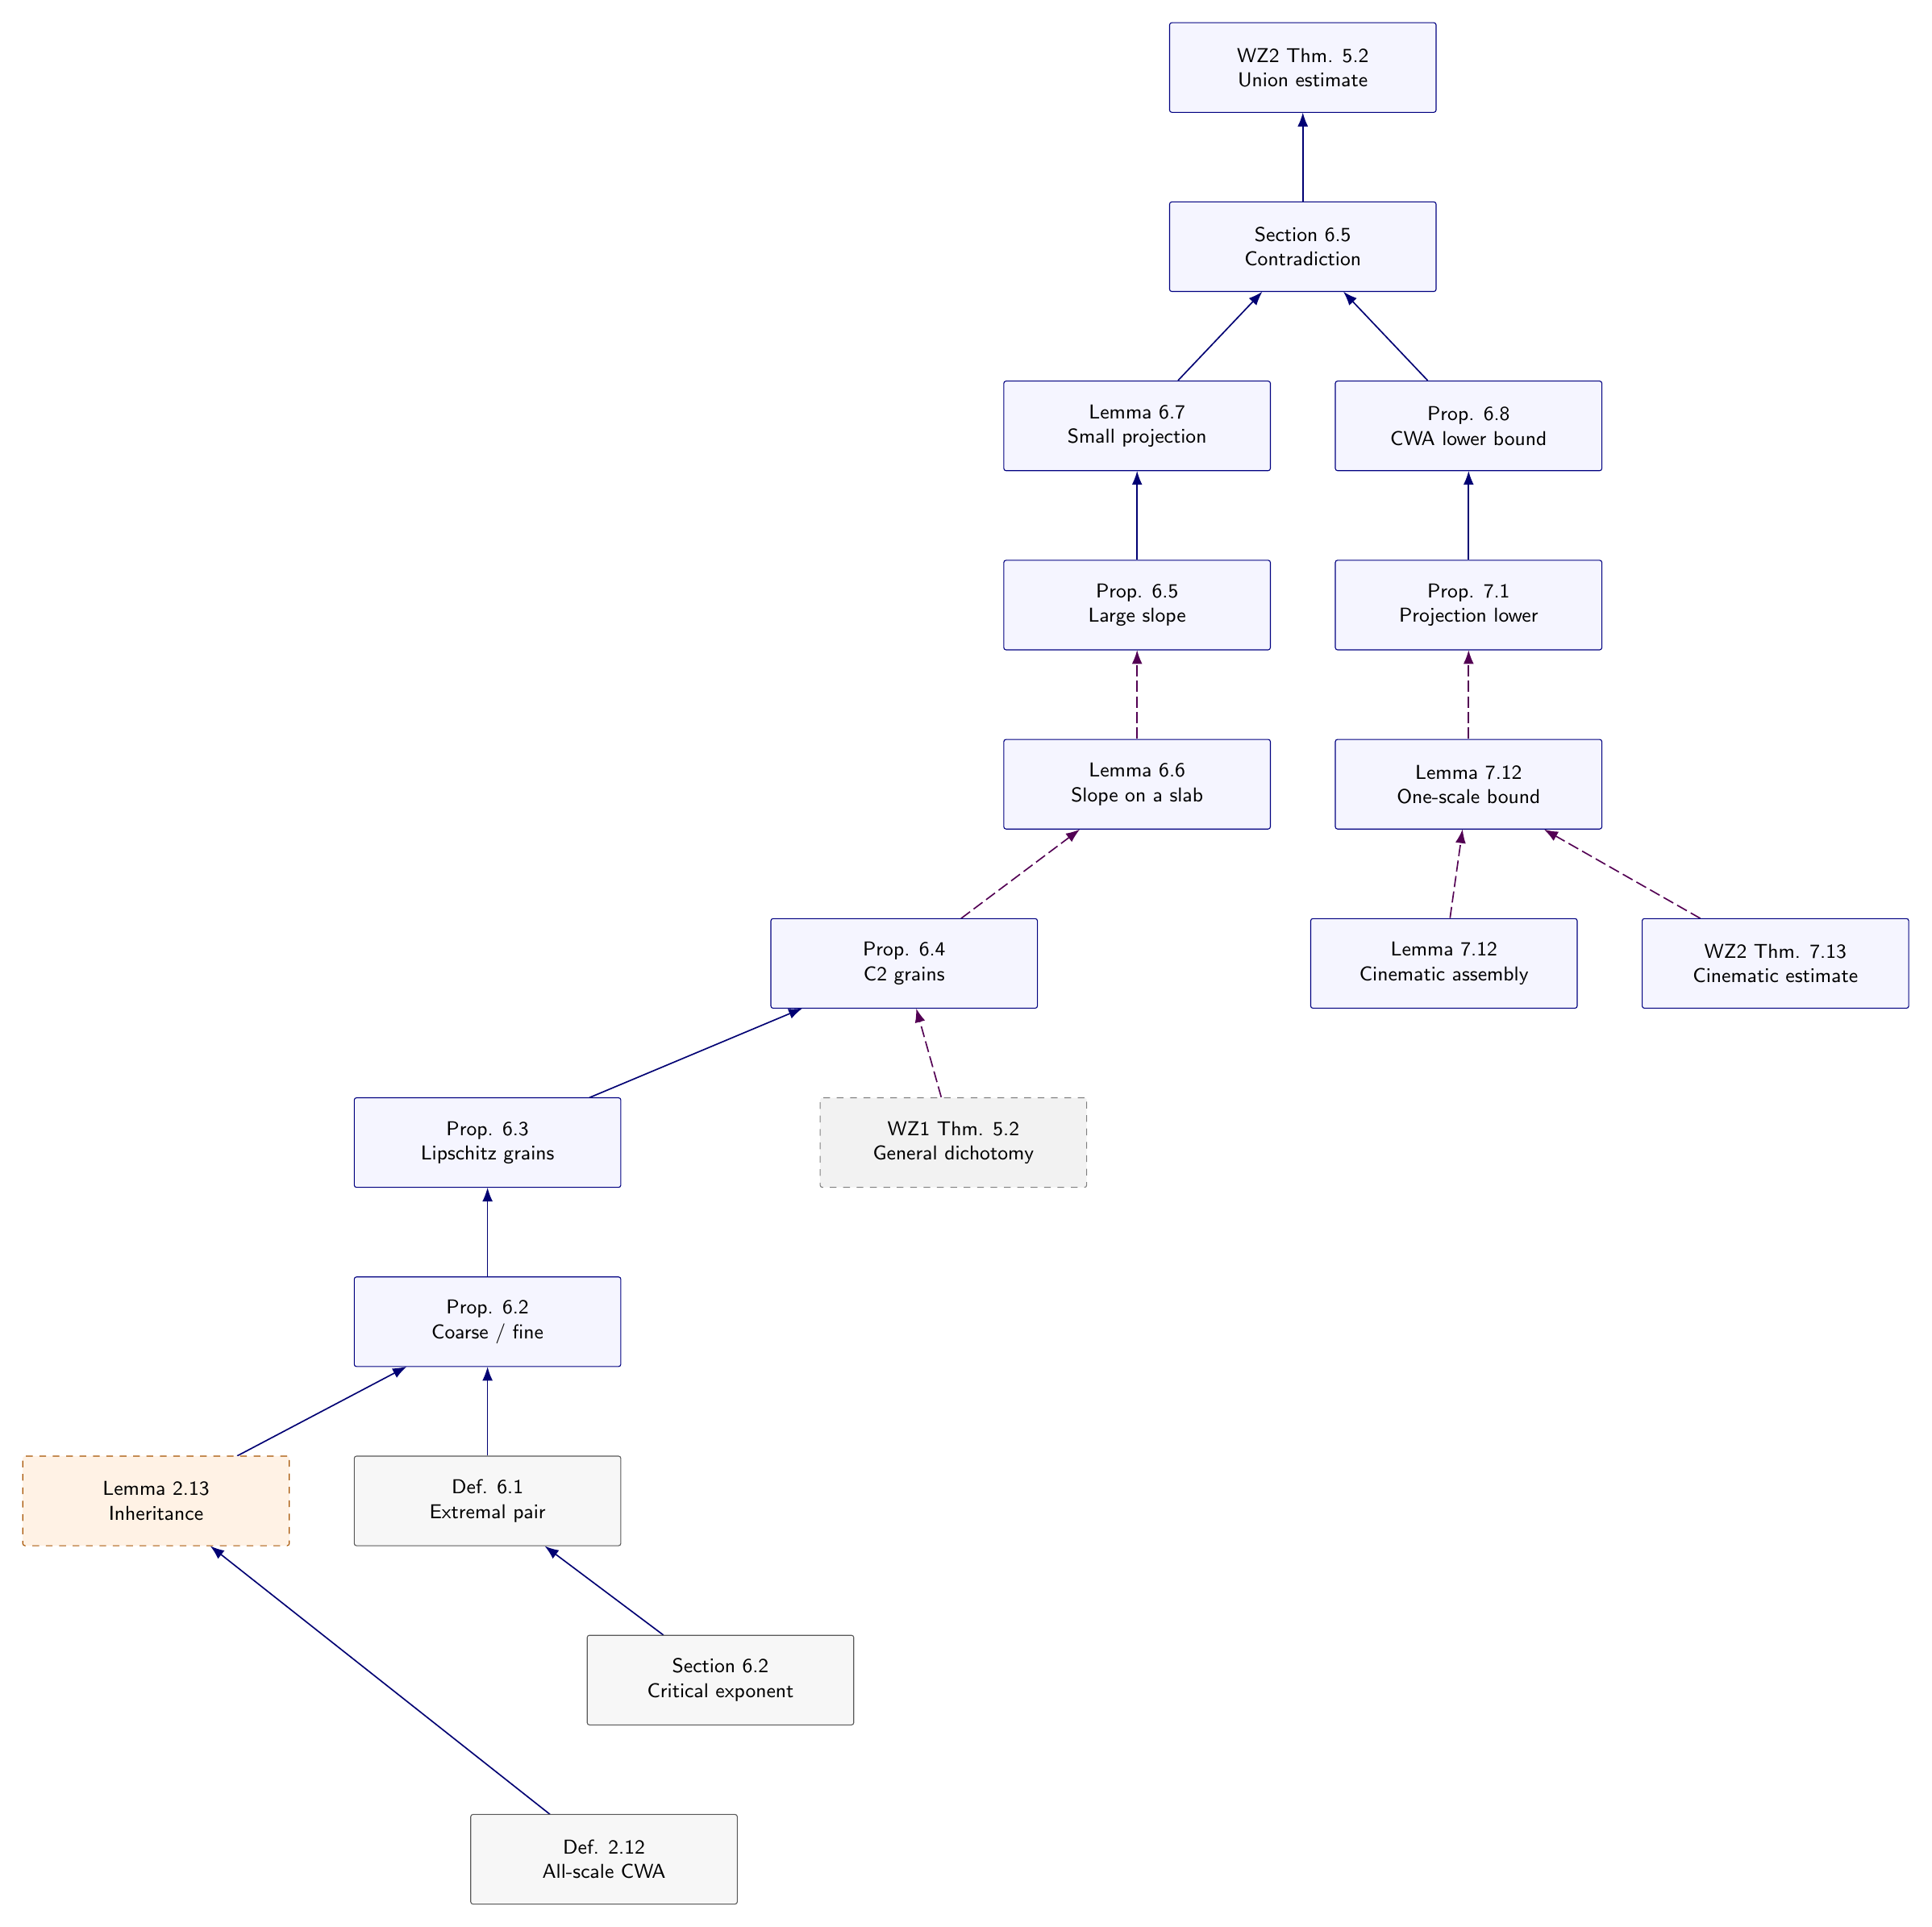
\begin{tikzpicture}[x=1cm,y=1cm,font=\sffamily\small]
\draw[-{Latex[length=2.2mm]},draw=blue!45!black,line width=.6pt] (8.30368,1.41323) .. controls (7.03474,2.41547) and (4.64573,4.30283) .. (3.23109,5.42043) -- (2.95310,5.63986);
\draw[-{Latex[length=2.2mm]},draw=blue!45!black,line width=.6pt] (10.09156,4.23616) .. controls (9.61637,4.59281) and (9.02617,5.03520) .. (8.51288,5.42008) -- (8.22113,5.63915);
\draw[-{Latex[length=2.2mm]},draw=blue!45!black,line width=.6pt] (3.37608,7.05838) .. controls (4.08693,7.43303) and (4.97769,7.90222) .. (5.73264,8.30016) -- (6.04696,8.46596);
\draw[-{Latex[length=2.2mm]},draw=blue!45!black,line width=.6pt] (7.32014,7.06543) .. controls (7.32014,7.37870) and (7.32014,7.75723) .. (7.32014,8.10436) -- (7.32014,8.46455);
\draw[-{Latex[length=2.2mm]},draw=blue!45!black,line width=.6pt] (7.32014,9.88766) .. controls (7.32014,10.20092) and (7.32014,10.57945) .. (7.32014,10.92659) -- (7.32014,11.28677);
\draw[-{Latex[length=2.2mm]},draw=blue!45!black,line width=.6pt] (8.92528,12.70282) .. controls (9.83827,13.08559) and (10.98797,13.56783) .. (11.94999,13.97141) -- (12.28196,14.11041);
\draw[-{Latex[length=2.2mm]},draw=violet!65!black,dash pattern=on 5pt off 2pt,line width=.6pt] (14.46601,12.70988) .. controls (14.37675,13.02632) and (14.26880,13.40979) .. (14.17003,13.76010) -- (14.07160,14.10899);
\draw[-{Latex[length=2.2mm]},draw=violet!65!black,dash pattern=on 5pt off 2pt,line width=.6pt] (14.77927,15.52504) .. controls (15.25446,15.88170) and (15.84466,16.32409) .. (16.35795,16.70897) -- (16.64970,16.92804);
\draw[-{Latex[length=2.2mm]},draw=violet!65!black,dash pattern=on 5pt off 2pt,line width=.6pt] (17.55069,18.35432) .. controls (17.55069,18.66759) and (17.55069,19.04612) .. (17.55069,19.39325) -- (17.55069,19.75344);
\draw[-{Latex[length=2.2mm]},draw=blue!45!black,line width=.6pt] (17.55069,21.17654) .. controls (17.55069,21.48981) and (17.55069,21.86834) .. (17.55069,22.21548) -- (17.55069,22.57566);
\draw[-{Latex[length=2.2mm]},draw=blue!45!black,line width=.6pt] (18.19592,23.99877) .. controls (18.52154,24.34202) and (18.92159,24.76359) .. (19.27542,25.13683) -- (19.52343,25.39788);
\draw[-{Latex[length=2.2mm]},draw=violet!65!black,dash pattern=on 5pt off 2pt,line width=.6pt] (22.47971,15.53210) .. controls (22.52380,15.84537) and (22.57707,16.22390) .. (22.62611,16.57103) -- (22.67691,16.93122);
\draw[-{Latex[length=2.2mm]},draw=violet!65!black,dash pattern=on 5pt off 2pt,line width=.6pt] (26.42270,15.52504) .. controls (25.77324,15.89476) and (24.96114,16.35725) .. (24.26794,16.75201) -- (23.95855,16.92804);
\draw[-{Latex[length=2.2mm]},draw=violet!65!black,dash pattern=on 5pt off 2pt,line width=.6pt] (22.77181,18.35432) .. controls (22.77181,18.66759) and (22.77181,19.04612) .. (22.77181,19.39325) -- (22.77181,19.75344);
\draw[-{Latex[length=2.2mm]},draw=blue!45!black,line width=.6pt] (22.77181,21.17654) .. controls (22.77181,21.48981) and (22.77181,21.86834) .. (22.77181,22.21548) -- (22.77181,22.57566);
\draw[-{Latex[length=2.2mm]},draw=blue!45!black,line width=.6pt] (22.12658,23.99877) .. controls (21.80096,24.34202) and (21.40091,24.76359) .. (21.04707,25.13683) -- (20.79907,25.39788);
\draw[-{Latex[length=2.2mm]},draw=blue!45!black,line width=.6pt] (20.16125,26.82099) .. controls (20.16125,27.13426) and (20.16125,27.51279) .. (20.16125,27.85992) -- (20.16125,28.22011);
\node[fill=gray!6,draw=gray!70!black,rounded corners=1pt,align=center,inner sep=1pt,minimum width=4.19811cm,minimum height=1.41112cm] at (9.15458,0.70556) {Def. 2.12\\All-scale CWA};
\node[fill=orange!10,draw=orange!65!black,dashed,rounded corners=1pt,align=center,inner sep=1pt,minimum width=4.19811cm,minimum height=1.41112cm] at (2.09903,6.35000) {Lemma 2.13\\Inheritance};
\node[fill=gray!6,draw=gray!70!black,rounded corners=1pt,align=center,inner sep=1pt,minimum width=4.19811cm,minimum height=1.41112cm] at (10.98903,3.52778) {Section 6.2\\Critical exponent};
\node[fill=gray!6,draw=gray!70!black,rounded corners=1pt,align=center,inner sep=1pt,minimum width=4.19811cm,minimum height=1.41112cm] at (7.32014,6.35000) {Def. 6.1\\Extremal pair};
\node[fill=blue!4,draw=blue!50!black,rounded corners=1pt,align=center,inner sep=1pt,minimum width=4.19811cm,minimum height=1.41112cm] at (7.32014,9.17222) {Prop. 6.2\\Coarse / fine};
\node[fill=blue!4,draw=blue!50!black,rounded corners=1pt,align=center,inner sep=1pt,minimum width=4.19811cm,minimum height=1.41112cm] at (7.32014,11.99444) {Prop. 6.3\\Lipschitz grains};
\node[fill=blue!4,draw=blue!50!black,rounded corners=1pt,align=center,inner sep=1pt,minimum width=4.19811cm,minimum height=1.41112cm] at (13.88181,14.81667) {Prop. 6.4\\C2 grains};
\node[fill=gray!10,draw=gray,dashed,rounded corners=1pt,align=center,inner sep=1pt,minimum width=4.19811cm,minimum height=1.41112cm] at (14.65792,11.99444) {WZ1 Thm. 5.2\\General dichotomy};
\node[fill=blue!4,draw=blue!50!black,rounded corners=1pt,align=center,inner sep=1pt,minimum width=4.19811cm,minimum height=1.41112cm] at (17.55069,17.63889) {Lemma 6.6\\Slope on a slab};
\node[fill=blue!4,draw=blue!50!black,rounded corners=1pt,align=center,inner sep=1pt,minimum width=4.19811cm,minimum height=1.41112cm] at (17.55069,20.46111) {Prop. 6.5\\Large slope};
\node[fill=blue!4,draw=blue!50!black,rounded corners=1pt,align=center,inner sep=1pt,minimum width=4.19811cm,minimum height=1.41112cm] at (17.55069,23.28333) {Lemma 6.7\\Small projection};
\node[fill=blue!4,draw=blue!50!black,rounded corners=1pt,align=center,inner sep=1pt,minimum width=4.19811cm,minimum height=1.41112cm] at (20.16125,26.10556) {Section 6.5\\Contradiction};
\node[fill=blue!4,draw=blue!50!black,rounded corners=1pt,align=center,inner sep=1pt,minimum width=4.19811cm,minimum height=1.41112cm] at (22.38375,14.81667) {Lemma 7.12\\Cinematic assembly};
\node[fill=blue!4,draw=blue!50!black,rounded corners=1pt,align=center,inner sep=1pt,minimum width=4.19811cm,minimum height=1.41112cm] at (22.77181,17.63889) {Lemma 7.12\\One-scale bound};
\node[fill=blue!4,draw=blue!50!black,rounded corners=1pt,align=center,inner sep=1pt,minimum width=4.19811cm,minimum height=1.41112cm] at (27.60486,14.81667) {WZ2 Thm. 7.13\\Cinematic estimate};
\node[fill=blue!4,draw=blue!50!black,rounded corners=1pt,align=center,inner sep=1pt,minimum width=4.19811cm,minimum height=1.41112cm] at (22.77181,20.46111) {Prop. 7.1\\Projection lower};
\node[fill=blue!4,draw=blue!50!black,rounded corners=1pt,align=center,inner sep=1pt,minimum width=4.19811cm,minimum height=1.41112cm] at (22.77181,23.28333) {Prop. 6.8\\CWA lower bound};
\node[fill=blue!4,draw=blue!50!black,rounded corners=1pt,align=center,inner sep=1pt,minimum width=4.19811cm,minimum height=1.41112cm] at (20.16125,28.92778) {WZ2 Thm. 5.2\\Union estimate};
\end{tikzpicture}%
}
\newcommand{\CoreLeanFigure}{%
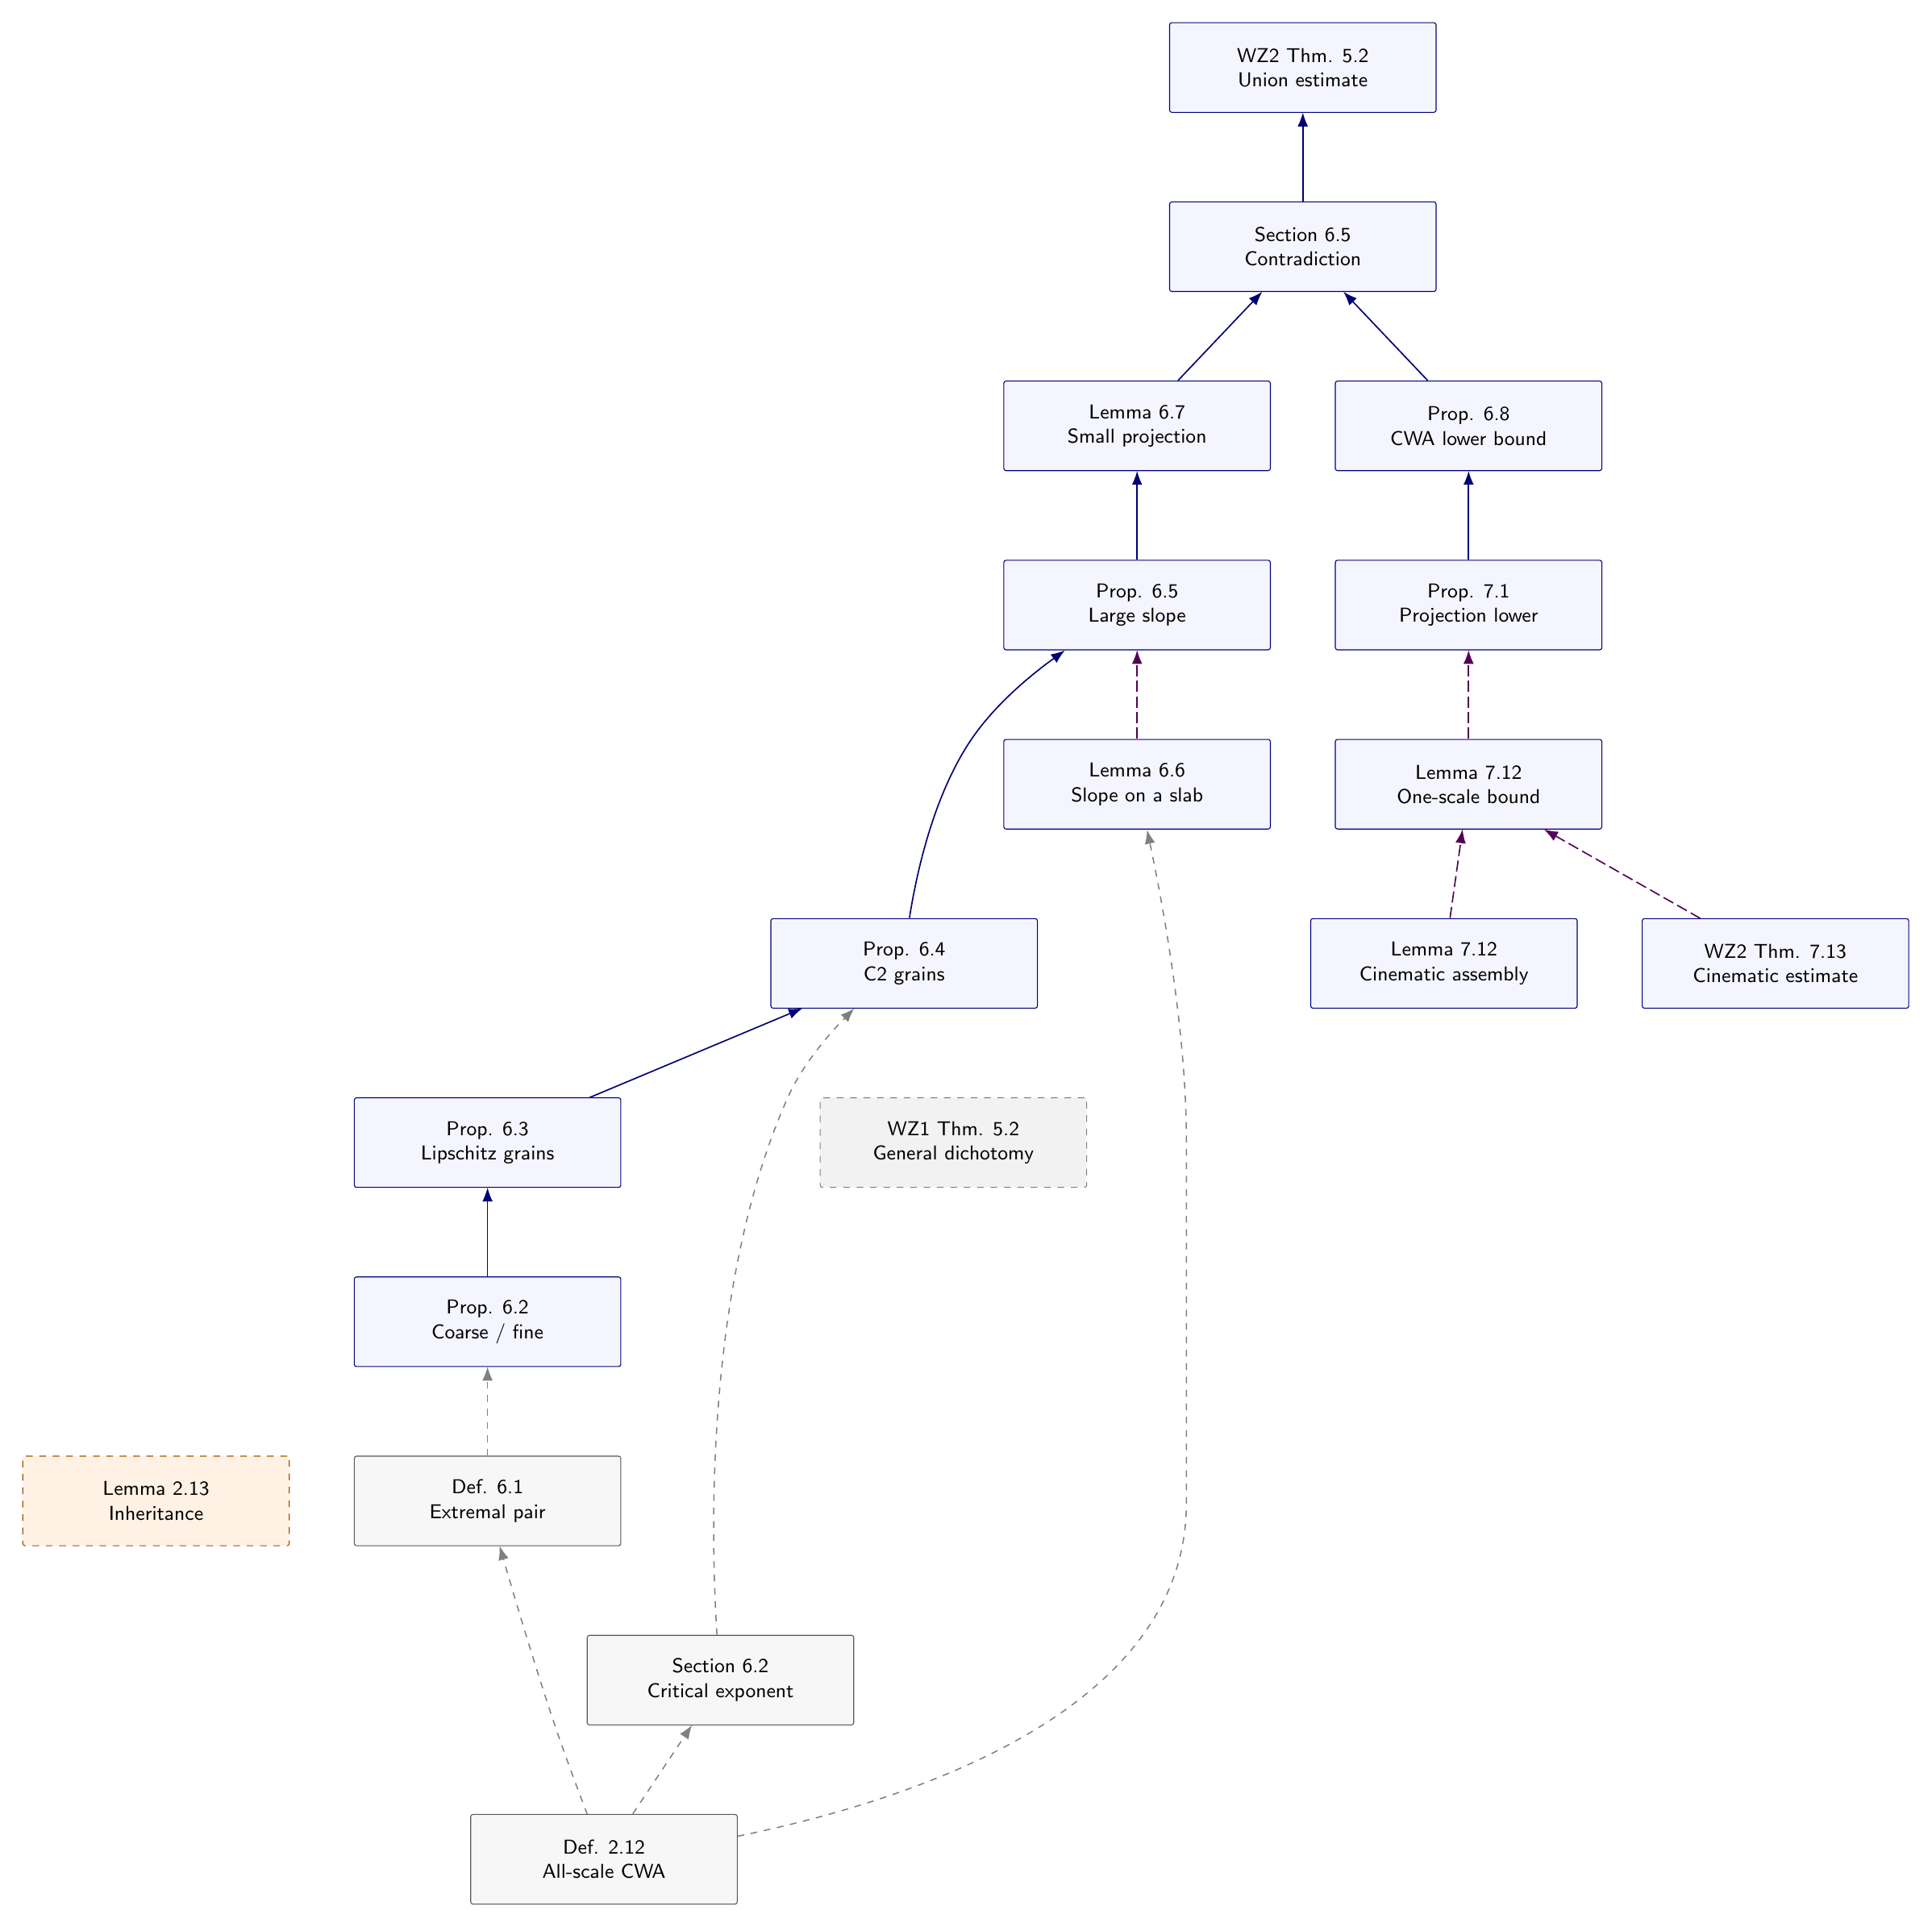
\begin{tikzpicture}[x=1cm,y=1cm,font=\sffamily\small]
\draw[-{Latex[length=2.2mm]},draw=gray,dashed,line width=.55pt] (9.60790,1.42099) .. controls (9.83015,1.75436) and (10.10144,2.16147) .. (10.34486,2.52624) -- (10.54065,2.82014);
\draw[-{Latex[length=2.2mm]},draw=blue!45!black,line width=.6pt] (20.16125,26.82099) .. controls (20.16125,27.13426) and (20.16125,27.51279) .. (20.16125,27.85992) -- (20.16125,28.22011);
\draw[-{Latex[length=2.2mm]},draw=gray,dashed,line width=.55pt] (8.89212,1.41182) .. controls (8.73654,1.81786) and (8.53899,2.34703) .. (8.37847,2.82222) .. controls (8.09907,3.65019) and (7.81332,4.60022) .. (7.60942,5.30013) -- (7.51064,5.64127);
\draw[-{Latex[length=2.2mm]},draw=blue!45!black,line width=.6pt] (22.77181,21.17654) .. controls (22.77181,21.48981) and (22.77181,21.86834) .. (22.77181,22.21548) -- (22.77181,22.57566);
\draw[-{Latex[length=2.2mm]},draw=gray,dashed,line width=.55pt] (10.93364,4.24109) .. controls (10.83381,5.80743) and (10.74173,9.76771) .. (12.04736,12.70000) .. controls (12.23398,13.11945) and (12.53596,13.51492) .. (12.84146,13.84653) -- (13.09652,14.10899);
\draw[-{Latex[length=2.2mm]},draw=blue!45!black,line width=.6pt] (8.92528,12.70282) .. controls (9.83827,13.08559) and (10.98797,13.56783) .. (11.94999,13.97141) -- (12.28196,14.11041);
\draw[-{Latex[length=2.2mm]},draw=blue!45!black,line width=.6pt] (13.96541,15.53422) .. controls (14.08324,16.27858) and (14.35347,17.47943) .. (14.94014,18.34444) .. controls (15.24952,18.80059) and (15.68909,19.20487) .. (16.11948,19.53295) -- (16.41440,19.74779);
\draw[-{Latex[length=2.2mm]},draw=violet!65!black,dash pattern=on 5pt off 2pt,line width=.6pt] (17.55069,18.35432) .. controls (17.55069,18.66759) and (17.55069,19.04612) .. (17.55069,19.39325) -- (17.55069,19.75344);
\draw[-{Latex[length=2.2mm]},draw=blue!45!black,line width=.6pt] (17.55069,21.17654) .. controls (17.55069,21.48981) and (17.55069,21.86834) .. (17.55069,22.21548) -- (17.55069,22.57566);
\draw[-{Latex[length=2.2mm]},draw=gray,dashed,line width=.55pt] (11.25890,1.06821) .. controls (13.96683,1.62243) and (18.32681,3.02577) .. (18.32681,6.31472) .. controls (18.32681,6.31472) and (18.32681,6.31472) .. (18.32681,12.02972) .. controls (18.32681,13.62745) and (18.01001,15.45802) .. (17.78141,16.57244) -- (17.70768,16.92134);
\draw[-{Latex[length=2.2mm]},draw=violet!65!black,dash pattern=on 5pt off 2pt,line width=.6pt] (22.47971,15.53210) .. controls (22.52380,15.84537) and (22.57707,16.22390) .. (22.62611,16.57103) -- (22.67691,16.93122);
\draw[-{Latex[length=2.2mm]},draw=violet!65!black,dash pattern=on 5pt off 2pt,line width=.6pt] (26.42270,15.52504) .. controls (25.77324,15.89476) and (24.96114,16.35725) .. (24.26794,16.75201) -- (23.95855,16.92804);
\draw[-{Latex[length=2.2mm]},draw=blue!45!black,line width=.6pt] (22.12658,23.99877) .. controls (21.80096,24.34202) and (21.40091,24.76359) .. (21.04707,25.13683) -- (20.79907,25.39788);
\draw[-{Latex[length=2.2mm]},draw=blue!45!black,line width=.6pt] (18.19592,23.99877) .. controls (18.52154,24.34202) and (18.92159,24.76359) .. (19.27542,25.13683) -- (19.52343,25.39788);
\draw[-{Latex[length=2.2mm]},draw=gray,dashed,line width=.55pt] (7.32014,7.06543) .. controls (7.32014,7.37870) and (7.32014,7.75723) .. (7.32014,8.10436) -- (7.32014,8.46455);
\draw[-{Latex[length=2.2mm]},draw=blue!45!black,line width=.6pt] (7.32014,9.88766) .. controls (7.32014,10.20092) and (7.32014,10.57945) .. (7.32014,10.92659) -- (7.32014,11.28677);
\draw[-{Latex[length=2.2mm]},draw=violet!65!black,dash pattern=on 5pt off 2pt,line width=.6pt] (22.77181,18.35432) .. controls (22.77181,18.66759) and (22.77181,19.04612) .. (22.77181,19.39325) -- (22.77181,19.75344);
\node[fill=gray!6,draw=gray!70!black,rounded corners=1pt,align=center,inner sep=1pt,minimum width=4.19811cm,minimum height=1.41112cm] at (9.15458,0.70556) {Def. 2.12\\All-scale CWA};
\node[fill=orange!10,draw=orange!65!black,dashed,rounded corners=1pt,align=center,inner sep=1pt,minimum width=4.19811cm,minimum height=1.41112cm] at (2.09903,6.35000) {Lemma 2.13\\Inheritance};
\node[fill=gray!6,draw=gray!70!black,rounded corners=1pt,align=center,inner sep=1pt,minimum width=4.19811cm,minimum height=1.41112cm] at (10.98903,3.52778) {Section 6.2\\Critical exponent};
\node[fill=gray!6,draw=gray!70!black,rounded corners=1pt,align=center,inner sep=1pt,minimum width=4.19811cm,minimum height=1.41112cm] at (7.32014,6.35000) {Def. 6.1\\Extremal pair};
\node[fill=blue!4,draw=blue!50!black,rounded corners=1pt,align=center,inner sep=1pt,minimum width=4.19811cm,minimum height=1.41112cm] at (7.32014,9.17222) {Prop. 6.2\\Coarse / fine};
\node[fill=blue!4,draw=blue!50!black,rounded corners=1pt,align=center,inner sep=1pt,minimum width=4.19811cm,minimum height=1.41112cm] at (7.32014,11.99444) {Prop. 6.3\\Lipschitz grains};
\node[fill=blue!4,draw=blue!50!black,rounded corners=1pt,align=center,inner sep=1pt,minimum width=4.19811cm,minimum height=1.41112cm] at (13.88181,14.81667) {Prop. 6.4\\C2 grains};
\node[fill=gray!10,draw=gray,dashed,rounded corners=1pt,align=center,inner sep=1pt,minimum width=4.19811cm,minimum height=1.41112cm] at (14.65792,11.99444) {WZ1 Thm. 5.2\\General dichotomy};
\node[fill=blue!4,draw=blue!50!black,rounded corners=1pt,align=center,inner sep=1pt,minimum width=4.19811cm,minimum height=1.41112cm] at (17.55069,17.63889) {Lemma 6.6\\Slope on a slab};
\node[fill=blue!4,draw=blue!50!black,rounded corners=1pt,align=center,inner sep=1pt,minimum width=4.19811cm,minimum height=1.41112cm] at (17.55069,20.46111) {Prop. 6.5\\Large slope};
\node[fill=blue!4,draw=blue!50!black,rounded corners=1pt,align=center,inner sep=1pt,minimum width=4.19811cm,minimum height=1.41112cm] at (17.55069,23.28333) {Lemma 6.7\\Small projection};
\node[fill=blue!4,draw=blue!50!black,rounded corners=1pt,align=center,inner sep=1pt,minimum width=4.19811cm,minimum height=1.41112cm] at (20.16125,26.10556) {Section 6.5\\Contradiction};
\node[fill=blue!4,draw=blue!50!black,rounded corners=1pt,align=center,inner sep=1pt,minimum width=4.19811cm,minimum height=1.41112cm] at (22.38375,14.81667) {Lemma 7.12\\Cinematic assembly};
\node[fill=blue!4,draw=blue!50!black,rounded corners=1pt,align=center,inner sep=1pt,minimum width=4.19811cm,minimum height=1.41112cm] at (22.77181,17.63889) {Lemma 7.12\\One-scale bound};
\node[fill=blue!4,draw=blue!50!black,rounded corners=1pt,align=center,inner sep=1pt,minimum width=4.19811cm,minimum height=1.41112cm] at (27.60486,14.81667) {WZ2 Thm. 7.13\\Cinematic estimate};
\node[fill=blue!4,draw=blue!50!black,rounded corners=1pt,align=center,inner sep=1pt,minimum width=4.19811cm,minimum height=1.41112cm] at (22.77181,20.46111) {Prop. 7.1\\Projection lower};
\node[fill=blue!4,draw=blue!50!black,rounded corners=1pt,align=center,inner sep=1pt,minimum width=4.19811cm,minimum height=1.41112cm] at (22.77181,23.28333) {Prop. 6.8\\CWA lower bound};
\node[fill=blue!4,draw=blue!50!black,rounded corners=1pt,align=center,inner sep=1pt,minimum width=4.19811cm,minimum height=1.41112cm] at (20.16125,28.92778) {WZ2 Thm. 5.2\\Union estimate};
\end{tikzpicture}%
}

\begin{figure}[p]
 \centering
 \resizebox{.98\textwidth}{!}{\CoreRoadmapFigure}
 \caption{Core 的 Roadmap 层：保留 18 个节点和原 17 条线。}
\end{figure}
\begin{figure}[p]
 \centering
 \resizebox{.98\textwidth}{!}{\CoreLeanFigure}
 \caption{Core 的 Lean 层：共 17 条线，含 12 对共同端点和另外 5 对端点。
 没有独立对应的 Lemma 2.13 和未使用的一般 WZ1 接口仍保留为节点。}
\end{figure}
\clearpage

\section{核对资料、证据及复查办法}

\subsection{数学卡片和源码来自哪里}

Core 的节点与 Roadmap 线来自 \path{blueprint/expert-atlas.json} 的
\id{overview} 视图。节点原始文字来自用户提供的
\path{artifacts/wz2_theorem_5_2_dependency_atlas.tex} 和对应 HTML；
blueprint 的导入器会核对两份文件的数学陈述。本文没有把里面的 Lean
伪代码当作编译证明。

各节点主声明、其他版本和范围说明来自
\path{blueprint/atlas-mapping.json}。本文逐项读了相应 Lean 定义、
证明入口和配置字段；它没有只把映射 Remark 翻译成中文。已编译
声明类型和引用证据来自 \path{blueprint/lean-declarations.json}、
\path{blueprint/lean-dependencies.json} 以及当前源码。

论文编号按 WZ2 \emph{The Assouad dimension of Kakeya sets in
$\R^3$} 的 arXiv 2401.12337v2 与该 Roadmap 使用的 WZ1 编号。
特别核对了 WZ2 式 (6.2)、(6.11)、Lemma 7.12 和 Theorem 7.13。
打印编号和源码模块内的旧节点编号不总相同，定位时优先使用本文给出的
声明名。

若要继续检查一般论文范围，直接看 blueprint 的
\id{rem:lemma66-mass-normalization}、\id{rem:projection-sign}、
\id{rem:parameter-frostman} 和 \id{rem:longitudinal-tube-model}。
它们分别记录绝对质量区别、上界符号、斜率与坐标归一化、粗轴长度修改。

\subsection{为什么依赖结论可复查}

配套的 \path{core-proof-dag-evidence.json} 对 18 个节点保留主声明、
源码位置、编译类型、证明／接口角色和根证明是否使用的信息；对全部
17 条 Roadmap 线保留分类与引用路径；对 17 条 Lean 线保留角色和
每一步引用类型。它还保留 C² 构造到已证明分离投影结果的路径。
引用步骤区分证明或定义的值、类型和结构引用。

\path{core-proof-dag-evidence.py} 可以从当前工作树重新生成该证据和
两幅 TikZ 图。这个脚本使用 blueprint 原有路径算法，Roadmap 边不会
进入 Lean 可达性计算。重新生成后应再检查数学陈述，而不是把分类器
当作证明两种陈述等价的工具。

本文写作期间，\path{blueprint/scripts/check.py} 的当前检查通过，
并重新编译了 \path{blueprint/scripts/core_contracts.lean}。后者检查
公共接口、同族 CWA、实际构造得到的配置的映射及上游参数使用。它们支持这里对
现有声明和输入关系的说明，但不能把一般打印版的缺口变成已证明结论。

\subsection{交给 Seed Evolving 时需要能复述的内容}

交接不是让另一个模型只说“看懂了”。它需要用自己的话说明至少这些
问题：为什么 C² 生产者和独立 Lemma 6.6 分别进入 Proposition 6.5；
为什么完整 WZ1 Theorem 5.2 接口没有成为 C² 的依赖；为什么归一化
质量不能删去 $\delta^2\#\T$；为什么 $f(0)=0$ 与纵向位置问题互相
独立；长度 32 改变的是粗测试而非细管；最后如何在同一个
$\T,Y,f$ 上先固定下界参数再构造上界。

它还需要分清三类状态：没有独立对应的节点、只定义了命题的节点、以及
证明了明确范围内版本的节点。连线比较的数字也应能复述：17 条 Roadmap
线中 12 条有路径，2 条无法用独立主声明比较，2 条是实际路线不同，
1 条涉及根证明外的接口；Lean 新画的 5 条 Core 直接线并不被分类器
标为 \emph{Lean only}。完整交接、它的复述及修订意见保存在配套
\path{core-proof-dag-seed-evolving-review.md}，以实际回复为准。

\end{document}


